\documentclass[12pt,a4paper]{article}
\usepackage[utf8]{inputenc}
\usepackage{dirtytalk}
\usepackage{csquotes}
\usepackage{hyperref}
\usepackage{graphicx}
\usepackage{amsmath}
\usepackage{amssymb}
\usepackage{eufrak}
\usepackage{float}
\floatplacement{figure}{H}
\floatplacement{table}{H}
\numberwithin{table}{section}
\numberwithin{figure}{section}
\numberwithin{equation}{section}

\title{Special and General Relativity}
\author{
  \textbf{\href{mailto:sreemanmohanreddy@gmail.com}{Kasi Reddy Sreeman Reddy}}\thanks{helped by my mentor Neel Singh}\\
  \texttt{Role No:190070029}
}
\date{April 2020}

\graphicspath{ {./images/} }
\usepackage[
    backend=biber, 
    natbib=true,
    style=numeric,
    sorting=none
]{biblatex}
\addbibresource{bibliography.bib}


\usepackage{amsthm}
%\newtheorem{theorem}{Theorem}
\newtheorem{theorem}{Theorem}[section]
\newtheorem{corollary}{Corollary}[theorem]
\newtheorem{lemma}[theorem]{Lemma}
\newtheorem{axiom}[theorem]{Axiom}

\theoremstyle{remark}
\newtheorem*{remark}{Remark}

\theoremstyle{definition}
\newtheorem{definition}{Definition}[section]
\renewcommand\qedsymbol{$\blacksquare$}


\usepackage{tensor}
\DeclareRobustCommand{\stirling}{\genfrac\{\}{0pt}{}}
\begin{document}
\maketitle
\begin{abstract}
First we are going to learn concepts of special theory of relativity from basic postulates. We then introduce Tensors and Tensor calculus and after that we deal with basic General Relativity. We are using the Einstein notation(1916) and not the new Abstract index notation of Penrose and Rindler(1984).
\end{abstract}
\tableofcontents
\section{Introduction to Special Relativity}
\subsection{Newtonian Relativity}

\begin{table}[h!]
\begin{center}
\begin{tabular}{|c|}

\hline
$x' = x-vt$  \\ 
$y' = y$\\  
$z' = z$\\ 
$t' = t$\\
\hline

\end{tabular}
\caption{Galilean Transformations}
 \label{table:1}

\end{center}
\end{table}
Newtonian Relativity(also called as Galilean invariance) is a Principle of relativity based on the \textbf{Galilean Transformations}($S'$ frame is moving toward right along x-axis with speed v wrt $S$) given in Table 1. Newtonian Relativity states that -
\begin{displayquote}
The laws of mechanics are \textbf{\textit{invariant}} under a \textbf{Galilean Transformation}.
\end{displayquote}
This Principle of relativity was initially stated only for laws of Mechanics. For centuries people believed in both Galilean Transformations and Newtonian Relativity.



\begin{table}[h!]
\begin{center}
\begin{tabular}{|c|}

\hline
$
\nabla \cdot \textbf{E}=\frac{\rho}{\epsilon_0}
$\\ 
$
\nabla \times \textbf{E}=- \frac{\partial \textbf{B}}{\partial t}
$\\  

$\nabla \cdot \textbf{B}=0
$\\
$c^2(\nabla \times \textbf{B})={\frac{j}{\epsilon_0}+\frac{\partial \textbf{E}}{\partial t}}$
\\
\hline

\end{tabular}
\caption{Maxwell's Equations}
 \label{table:1}

\end{center}
\end{table}
Table 2 contains Maxwell's equations which when combined with Lorentz force law($\textbf{F}=q(\textbf{E} +\textbf{v} \times \textbf{B} )$) explains us Electrodynamics. These equations predicted that the speed of electromagnetic waves is c (around $3\times 10^8m/s$). Since most of the waves then known used to propagate through some medium they assumed it is the speed in through a medium which was named as ether.  But after this there were some inconsistencies with classical mechanics in electrodynamics phenomena. So they came up with these 3 possibilities

\begin{enumerate}
  \item A relativity principle exists for mechanics, but \textbf{not} for electrodynamics; in electrodynamics there is a preferred inertial frame; that is,the ether frame. If this alternative is correct the Galilean transformations would apply and we would be able to locate the ether frame 
experimentally.

  \item A relativity principle exists both for mechanics and for electrodynamics, but the laws of electrodynamics as given by Maxwell are not 
correct. The Galilean transformations 
would apply here also.
  \item A relativity principle exists both for mechanics and for electrodynamics, but the Galilean transformations and the laws of mechanics as given by Newton are not correct. 

\end{enumerate}
People proposed a lot of different theories to make them consistent. Among them \textbf{Lorentz, Fitzgerald} and \textbf{Larmor} used complex and wrong arguments and got correct equations which are now called Lorentz transformations. Although they got the correct equations what they understood from that was wrong. \textbf{Poincaré} based on \textbf{Michelson–Morley} experiment suggested that the ether theories are wrong and he opted for the 3rd option. But none of them succeeded except  \textbf{Albert Einstein} who also chose the 3rd option and created his  \textbf{Special Relativity} which was later verified to be true. The biggest success of Einstein was that he thought that  \textbf{time} may not be  \textbf{absolute}. In fact the forth equation in Galilean transformations was never explicitly written because it was assumed to be obvious. But Newton still explicitly wrote it in his \textbf{\textit{Principia}} -
\begin{displayquote}
Absolute, true and mathematical time, of itself, and from its own nature flows equably without regard to anything external, and by another name is called duration.
\end{displayquote}

Einstein's Special Relativity was made from these 2 postulates- 
\begin{enumerate}
  \item The laws of physics are the same in all inertial systems. No preferred 
inertial frame exists.(Notice \textbf{not} just laws of Mechanics) 

  \item The speed of light in free space has the same value c in all inertial 
systems. 

\end{enumerate}
\begin{figure}[H]
    \centering
  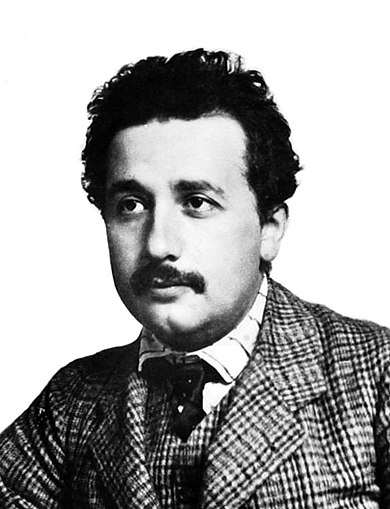
\includegraphics[scale=0.25]{Einstein}
  \caption{Einstein around 1905(Source:Wikipedia)}
  \label{fig:Einstein}
\end{figure}

\subsection{The Relativity of Simultaneity}
\textbf{Synchronisation of clocks}: When we say a \textbf{reference frame} we are referring to imaginary clocks which are point sized and are everywhere in the universe and sticks which are at 1m length(in that frame). Now to synchronize all these clocks we send light signals from a point clock when it is set to $t=0$ to all other clocks and other clock are set such that if they are at a distance of r from the point then they are set to $t=r/c$.
We define measurement of length as the difference between coordinates at an single instant.
\begin{figure}[H]
    \centering
  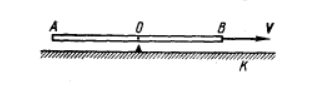
\includegraphics[scale=1]{2}
  \caption{wrt $S$ frame(source:Fundamental laws of Mechanics)}
  \label{fig:2}
\end{figure}

Imagine a rod moving along x-axis in $S$ frame with same speed as $ S'$ as shown in figure 2. Now let a light pulse be ejected from the middle point O. Then wrt $K$ frame it will touch A first and then B because it travel at the speed of c and point A is moving towards O. But in $S'$ frame it touches both frames at the same time since A and B are at rest.So, \textbf{simultaneity is relative}.


\subsection{Deriving the Lorentz Transformations}
An event is characterized by co-ordinates of space and time in a reference frame. Let an event be characterized ${x',y',z',t'}$ in $S'$ and ${x,y,z,t}$ in $S$. We are assuming that space is isotropic and homogeneous. So there is no preferred angle. If the equations are non linear then it would violate the homogeneity. So, the most general transformations are(all coefficients are only functions of v)-
\begin{center}
$x' = a_{ll}x + a_{l2}y + a_{l3}z + a_{l4}t$\\
$y' = a_{2l}x + a_{22}y + a_{23}z + a_{24}t$\\
$z' = a_{3l}x + a_{32}y + a_{33}z + a_{34}t$\\
$t' = a_{4l}x + a_{42}y + a_{43}z + a_{44}t$\\
\end{center}

If $v=0$ then both frames coincide so $a_{ll},a_{22},a_{33} and a_{44}$ are equal to 1 when $v=0$.

The $x$-axis coincides continuously with the $x'$-axis. This will be so 
only if for $y = 0$, $z = 0$ (which characterizes points on the x-axis) it 
always follows that $y' = 0$, $z' = 0$ (which characterizes points on the 
x'-axis). Hence, the transformation formulas for y and z must be of the 
form 
\begin{center}
$y' = a_{22}y + a_{23}z$\\
$z' = a_{32}y + a_{33}z$\\
\end{center}
similarly, for the $x-z$ and $x' -z'$ planes, $y = 0$ should give $y' = O$. Hence, it follows that $a_{23}$ and $a_{32}$  are zero so that
\begin{center}
$y' = a_{22}y$\\
$z' = a_{33}z$\\
\end{center}

Now imagine a rod on $y$-axis between origin and $y=1m$. It's length will be $a_{22}$ in $S'$ frame. Now let there be a 1m in $S'$ frame which in $s$ fram will have length $\frac{1}{a_{22}}$. Now because of 1st postulate these two should be equal because both are 1m length rods and are observed by a frame moving at speed $v$. So, $a_{22}=\frac{1}{a_{22}} $. So $a_{22}=1$. Similarly $a_{33}=1$ .$a_{42}$ and $a_{43}$ have to be $0$. Otherwise, clocks placed symmetrically in the y-z plane (such as at +y, -y or +z, -z) about the x-axis would appear to disagree as observed from $S'$, which would contradict 
the isotropy of space. We know that a point having $x'=0$ appears to move in the direction of the positive x-axis with speed v, so that the statement $x' = 0$ must be identical to the statement $x = vt$. So, they are reduced to

\begin{center}
$x' = a_{11}(x-vt)$\\
$y' = y$\\
$z' = z$\\
$t' = a_{41}x + a_{44}t$\\
\end{center}
Now we can use the 2nd postulate.Let us assume that at the time t = 0 a spherical electromagnetic wave leaves the origin of $S$, which coincides with the origin of $S'$ at that moment. The wave propagates with a speed c in all directions in each inertial frame. Its progress, then, is described by the equation of sphere whose radius expands with time at a rate c in terms of either the primed or unprimed set of coordinates. That is, 

\begin{center}
$x^2 + y^2 + z^2 = c^2t^2$\\
$x'^2 + y'^2 + z'^2 = c^2t'^2$\\
\end{center}
If we now substitute the 4 transformations in the above equation for the primed coordinates we get
\begin{center}
$a_{11}(x-vt)^2 + y^2 + z^2 = c^2(a_{41}x + a_{44}t)$\\
$\Rightarrow (a_{11}^2-c^2a_{41}^2)x^2 + y^2 + z^2 - 2(va_{11}^2+c^2a_{41}a_{44}) = (c^2a_{44}^2-v^2a_{11}^2)t^2$\\
\end{center}
which gives

\begin{center}
$a_{11}^2-c^2a_{41}^2=1$\\
$va_{11}^2+c^2a_{41}a_{44}=0$\\
$c^2a_{44}^2-v^2a_{11}^2=c^2$\\
\end{center}
On solving we get
\begin{equation}
    x'=\frac{x-vt}{ \sqrt{1-(\frac{v}{c})^2}}
\end{equation}
\begin{equation}
    y'=y
\end{equation}
\begin{equation}
    z'=z
\end{equation}
\begin{equation}
    t'=\frac{t-\frac{v}{c^2}x}{\sqrt{1-(\frac{v}{c})^2}}
\end{equation}

The equations 1 to 4 are referred to as Lorentz transformations. We can also find the reverse equations for them by solving equations 1 and 4. Notice that we get $-v$ instead of $v$ as expected. 
\begin{table}[H]
\begin{center}
\begin{tabular}{||c|c||}
\hline
From $S$ to $S'$ & From $S'$ to $S$\\
\hline
$ x'=\dfrac{x-vt}{ \sqrt{1-(\dfrac{v}{c})^2}}$ & $ x=\dfrac{x'+vt'}{ \sqrt{1-(\dfrac{v}{c})^2}}$\\ 
$y' = y$ & $y = y'$\\  
$z' = z$ & $z = z'$\\ 
$t' = \dfrac{t-\dfrac{v}{c^2}x}{\sqrt{1-(\dfrac{v}{c})^2}}$ & $t = \dfrac{t'+\dfrac{v}{c^2}x'}{\sqrt{1-(\dfrac{v}{c})^2}}$\\
\hline

\end{tabular}
\caption{Lorentz Transformations}
 \label{table:3}
 
\end{center}
\end{table}


The Lorentz transformations reduce to the Galilean transformations in the limit  $c \to \infty $ or $\frac{v}{c}<<1$
\subsection{Simple consequences of Lorentz transformations}
The Lorentz Transformations have many beautiful consequences some of them are:
\subsubsection{Lorentz contraction}
Let there be a rod in $S$ frame along $x$-axis form ($x_1$,0,0) to ($x_2$,0,0)
Form this we get 
\begin{center}
$ x'_1=\dfrac{x_1-vt_1}{ \sqrt{1-(\dfrac{v}{c})^2}}$  $ x'_2=\dfrac{x_2-vt_2}{ \sqrt{1-(\dfrac{v}{c})^2}}$
$\Rightarrow x_2'-x_1'=\dfrac{x_2-x_1-v(t_2-t_1)}{\sqrt{1-(\dfrac{v}{c})^2}}$

\end{center}
But we measure the length of rod in $S$ in a single instant. So $t_2=t_1$ and we get
\begin{center}
$x_2'-x_1'=\dfrac{x_2-x_1}{\sqrt{1-(\dfrac{v}{c})^2}}$
\end{center}
So the length is contracted along the direction of motion only. Also we call the length of an object measured in a frame in which it is at rest as \textbf{Proper length}(\textbf{$l_0$}). We define $\gamma=\frac{1}{\sqrt{1-(\dfrac{v}{c})^2}}$ and $\beta=\frac{v}{c}$. In all other frames it's length will be contracted in the $x$ direction by a factor of $\gamma$.
\begin{center}
$l=\dfrac{l_0}{\gamma}$
\end{center}
We tend to think that the relativistic length contraction would cause rapidly moving objects to appear to the eye to be shortened in the direction of motion. The location of all points of the object measured at the same time would give the "true" picture according to our use of the term "observer" in relativity. In the words of V. F. Weisskopf

\say{When we see or photograph an object, we record light quanta emitted 
by the object when they arrive simultaneously at the retina or at the 
photographic film. This implies that these light quanta have not been 
emitted simultaneously by all points of the object. The points further 
away from the observer have emitted their part of the picture earlier 
than the closer points. Hence, if the object is in motion, the eye or the 
photograph gets a distorted picture of the object, since the object has 
been at different locations when different parts of it have emitted the 
light seen in the picture.}


\subsubsection{Time dilation}
Let there be some event going on the point ($x,y,z$) from $t_1$ to $t_2$
Let $t_1',t_2'$ be the corresponding in $S'$ then
\begin{center}
$t_1' = \dfrac{t_1-\dfrac{v}{c^2}x}{\sqrt{1-(\dfrac{v}{c})^2}}$ and $t_2' = \dfrac{t_2-\dfrac{v}{c^2}x}{\sqrt{1-(\dfrac{v}{c})^2}} \Rightarrow$ $t_2'-t_1'= \dfrac{t_2-t_1}{\sqrt{1-(\dfrac{v}{c})^2}}$
\end{center}

So we can observe that time interval measured in the frame where the event is happening at a single place is the smallest interval and is called \textbf{Proper time}(d$\tau$) and time interval in some other frame is given by
\begin{center}
    $\Delta t=\gamma \Delta\tau$
\end{center}
Example 1: If a pion has proper life time = $1.77\times10^-8s$ and it's velocity relative to the lab is 0.99c. Then calculate the distance travelled by it in the lab frame.

Sol=
\begin{center}
$\Delta\tau=1.77\times10^-8s$\\
$\Delta t=\gamma \Delta\tau \Rightarrow \Delta t\approx1.3\times10^-7s$\\
$d=v\Delta t\approx39m$

\end{center}
\subsection{The relativistic addition of velocities }
From the Galilean transformations we can simply deduce $ \textbf{u=u'+v} $. Now we have to generalize it. We \textbf{define} velocity of an object in a frame as change in distance by change in time both observed in the \textbf{same reference frame} .From Lorentz equations we get
\begin{center}
 $dx=\gamma_v(dx'+vt'), dt=dy',dz=dz' $\\
 
 $\Rightarrow \dfrac{dx}{dt}=\dfrac{\gamma_v(dx'+vt')}{\gamma_v(dt'+\dfrac{v}{c^2}dx')}$,
 $\dfrac{dy}{dt}=\dfrac{dy'}{\gamma_v(dt'+\dfrac{v}{c^2}dx')}$,
 $\dfrac{dz}{dt}=\dfrac{dz'}{\gamma_v(dt'+\dfrac{v}{c^2}dx')}$
 
 
 $\Rightarrow u_x=\dfrac{\dfrac{dx'}{dt'}+v}{1+\dfrac{v}{c^2}\dfrac{dx'}{dt'}}$,
 $ u_y= \dfrac{\dfrac{dy'}{dt'}}{\gamma_v(1+\dfrac{v}{c^2}\dfrac{dx'}{dt'})}$,
$ u_z= \dfrac{\dfrac{dz'}{dt'}}{\gamma_v(1+\dfrac{v}{c^2}\dfrac{dx'}{dt'})}$\\
\end{center}

Example 2: Let a photon be moving at the speed of c along $x'$ axis  in $S'$ frame find it's speed with respect to $S$.
Sol:\begin{center}
    $u_x'=c$ \\
    $u_x=\dfrac{u_x'+v}{1+\dfrac{v}{c^2}u_x'}$\\
    $u_x=\dfrac{c+v}{1+\dfrac{v}{c^2}c}$\\
    
    $u_x=c$\\
\end{center}
This is what we expect since this is our postulate. In the general case where the light pulse is along some random direction it still maintains it's speed c in other frames but the \textbf{ direction} will change.

\begin{table}[H]
\begin{center}
\begin{tabular}{||c|c||}
\hline
From $S$ to $S'$ & From $S'$ to $S$\\
\hline
$u_x'=\dfrac{u_x-v}{1-\dfrac{v}{c^2}u_x}$ &
$u_x=\dfrac{u_x'+v}{1+\dfrac{v}{c^2}u_x'}$\\ & \\

$u_y'= \dfrac{u_y}{\gamma_v(1-\dfrac{v}{c^2}u_x)}$ &
$u_y= \dfrac{u_y'}{\gamma_v(1+\dfrac{v}{c^2}u_x')}$\\ & \\

$u_z'= \dfrac{u_z}{\gamma_v(1-\dfrac{v}{c^2}u_x)}$ &
$u_z= \dfrac{u_z'}{\gamma_v(1+\dfrac{v}{c^2}u_x')}$\\ & \\
\hline
\end{tabular}
\caption{Relativistic relative velocity}
 \label{table:4}
\end{center}
\end{table}





\subsection{Aberration and Doppler Effect in Relativity}
Let plane monochromatic light waves of unit amplitude  be emitted from a source at the origin of the $S'$-frame making an angle $\theta$ with the $x'$-axis and the normals being perpendicular t $x'-y'$plane, with the below equation()
\begin{center}
$\cos{2\pi(\dfrac{x'\cos{\theta'}+y'\sin{\theta}}{\lambda'}-\nu't')} $
\end{center}
We know that $\lambda'v'=c$. Let $\theta and \lambda$  be it's values in the $S$ frame. In the $S$ frame it's equation will be-

\begin{center}
$\cos{2\pi(\dfrac{x\cos{\theta}+y\sin{\theta}}{\lambda}-\nu t)} $
\end{center}
Now substituting Lorentz transformations in the first wave equation-

\begin{center}
$\cos{2\pi(\dfrac{\dfrac{x-vt}{ \sqrt{1-\beta^2}}\cos{\theta'}+y\sin{\theta}}{\lambda'}-\nu'(\dfrac{t-\dfrac{v}{c^2}x}{\sqrt{1-\beta^2}}))} $\\
$\Rightarrow$
$\cos{2\pi(\dfrac{\cos{\theta'}+\beta}{\lambda'\sqrt{1-\beta^2}}x+\dfrac{\sin{\theta'}}{\lambda'}y-\dfrac{\beta\cos{\theta'}+1}{\sqrt{1-\beta^2}}\nu't)} $

\end{center}
By comparing with the 2nd wave equation we get-
\begin{center}



$\dfrac{\cos{\theta'}+\beta}{\lambda'\sqrt{1-\beta^2}}=\dfrac{\cos{\theta}}{\lambda}$ \\
$\dfrac{\sin{\theta'}}{\lambda'}=\dfrac{\sin{\theta}}{\lambda} $\\
$\dfrac{\beta\cos{\theta'}+1}{\sqrt{1-\beta^2}}\nu'=\nu$\\

\end{center}
On solving these 3 we get-

\begin{equation}
\tan\theta =\dfrac{\sin{\theta'}\sqrt{1-\beta^2}}{\cos{\theta'}+\beta}
\end{equation}


\begin{equation}
\nu= \nu'(\dfrac{1+\beta\cos{\theta'}}{\sqrt{1-\beta^2}})
\end{equation}
As usual you can get the equations for the other frame by replacing the sign of $\beta$. They are
\begin{equation}
\tan\theta' =\dfrac{\sin{\theta}\sqrt{1-\beta^2}}{\cos{\theta}-\beta}
\end{equation}


\begin{equation}
\nu'= \nu(\dfrac{1-\beta\cos{\theta}}{\sqrt{1-\beta^2}})
\end{equation}
The above frequency formula has far reaching consequences. Notice that unlike classical Doppler effect which depends both on the source speed and the observer speed with respect to medium, the \textbf{relativistic doppler effect} depends \textbf{only} on their \textbf{relative velocity.}

\section{Dynamics of Special Relativity}
\subsection{Momentum}
If we just use the old formula to define the momentum when we change frames the momentum of the particle will change. But we can redefine momentum such that momentum conservation is applicable. We define it as-
\begin{equation}
\textbf{P}=\dfrac{m_o\textbf{u}}{\sqrt{1-\beta^2}} 
\end{equation}


The reason we wrote $m_0$ instead of $m$ is in SR we have 2 kinds of masses
and we call this as the \textbf{rest mass or proper mass}. We define another mass known as  rest \textbf{relativistic mass} as $m=\dfrac{m_0}{\sqrt{1-\beta^2}} $. \textbf{Mass} is an ambiguous term in SR. Some call \textbf{rest mass} as mass and some call \textbf{relativistic mass} as mass. We use the later. Also $m$ and $m_0$ are related as
\begin{equation}
   m^2c^4=m_0^2c^4+p^2c^2
\end{equation}

We redefine Newton's second law as-
\begin{equation}
\textbf{F}=\dfrac{d\textbf{p}}{dt}=\dfrac{d(\dfrac{m_o\textbf{u}}{\sqrt{1-\beta^2}})}{dt}
\end{equation}
\subsection{Energy}
We define \textbf{Kinetic Energy} as
\begin{center}
    $K= \int_{u=0}^{u=u}\textbf{F}\cdot{d\textbf{l}}$\\
    $\Rightarrow K= \int_{u=0}^{u=u}\dfrac{d(mu)}{dt}\cdot{d\textbf{l}}$\\
\end{center}
Consider 1d motion. Then it reduces to
\begin{center}  
    $\Rightarrow K= \int_{u=0}^{u=u}\dfrac{d(mu)}{dt}\cdot{dx}$\\
    $\Rightarrow K= \int_{u=0}^{u=u}d(mu)\cdot\dfrac{dx}{dt}$\\
    $\Rightarrow K= \int_{u=0}^{u=u}(dmu+mdu)\cdot du $\\
\end{center}
Using equation 10 we get\\
\begin{equation}
K=\int_{m=m_0}^{m=m}c^2dm=mc^2-m_0c^2
\end{equation}
This equation suggests us that $m$ is a \textbf{measure} of energy. We define rest energy as $m_0c^2$ and total energy as $mc^2$. This formula again has many far reaching consequences. Although \textbf{Poincaré} first considered photon's energy and mass are interconnected it was \textbf{Einstein} who said this is true for all objects. Further it was proved experimentally many times. Even in day to day \textbf{chemical reactions} some mass is being converted to energy. But it can be easily detectable in case of \textbf{nuclear reactions}. So conservation of energy and mass are now united.
\begin{equation}
    E=mc^2
\end{equation}
\begin{equation}
    E^2=(pc)^2+(m_0c^2)
\end{equation}
We also get the below equation for E.
\begin{equation}
    \dfrac{dE}{dp}=u
\end{equation}

\subsection{Single particle dynamics}
\begin{center}
    $\textbf{F}=\dfrac{d\textbf{p}}{dt}=\dfrac{\dfrac{d(E\textbf{u})}{c^2}}{dt}$
\end{center}
On solving we get-
\begin{equation}
    \textbf{F}=m\dfrac{d\textbf{u}}{dt}+\dfrac{{\textbf{u}(\textbf{F}\cdot\textbf{u})}}{c^2}
\end{equation}
 
The acceleration(defined as $\dfrac{d\textbf{u}}{dt}$)in general is not parallel to the force  which is the case in classical mechanics.
\subsection{The Transformation Properties of Momentum, Energy, Mass, and 
Force}
We can just take momentum and force in one frame and then we can find the particle's dynamics. We then use particle's kinematical properties in the new frame and deduce the transformation laws. They are given in table 2.1 and 2.2
\begin{table}[H]
\begin{center}
\begin{tabular}{||c|c||}
\hline
From $S$ to $S'$ & From $S'$ to $S$\\
\hline
\\ & \\
$p_x'=\dfrac{p_x-\frac{Ev}{c^2}}{\sqrt{1-\dfrac{v}{c^2}}}$ &
$p_x=\dfrac{p_x'+\frac{E'v}{c^2}}{\sqrt{1-\dfrac{v}{c^2}}} $\\ & \\

$p_y'= p_y$ &
$p_y= p_y' $\\ & \\

$p_z'=p_z$ &
$p_z=p_z' $\\ & \\
\hline
\end{tabular}
\caption{Relativistic momentum transformation}
 \label{table:4}
\end{center}
\end{table}
\begin{table}[H]
\begin{center}
\begin{tabular}{||c|c||}
\hline
From $S$ to $S'$ & From $S'$ to $S$\\
\hline
\\ & \\
$F_x'=F_x-\frac{u_yv}{c^2-u_xv}F_y-\frac{u_zv}{c^2-u_xv}F_z$ &
$F_x=F_x'+\frac{u_yv}{c^2+u_x'v}F_y'+\frac{u_zv}{c^2+u_x'v}F_z' $\\ & \\

$F_y'= \frac{\sqrt{1-\frac{v^2}{c^2}}}{1-\frac{u_xv}{c^2}}F_y$ &
$F_y= \frac{\sqrt{1-\frac{v^2}{c^2}}}{1+\frac{u_x'v}{c^2}}F_y' $\\ & \\

$F_z'= \frac{\sqrt{1-\frac{v^2}{c^2}}}{1-\frac{u_xv}{c^2}}F_z$ &
$F_z= \frac{\sqrt{1-\frac{v^2}{c^2}}}{1+\frac{u_x'v}{c^2}}F_z' $\\ & \\
\hline
\end{tabular}
\caption{Relativistic momentum transformation}
 \label{table:4}
\end{center}
\end{table}


\subsection{Need for a relativistic gravitation theory}
A very important formulation of Special relativity was done by \textbf{Hermann Minkowski}(he was a maths professor to Einstein) in 1907(2 years after Einstein).It is given in the next chapter. It was a geometrical approach to SR using tensors and other things which we will learn later. Einstein initially argued that it was \textbf{not necessary} to include all that maths since it can be understood simply.

Special Relativity explained us only about inertial frames. In Galilean relativity we know that if we transform to a non-inertial frame we have to consider Fictitious force and they are directly proportional to the mass of an object. Newton was well aware of the fact that the gravitational mass may be only approximately equal to the inertial mass. Where the masses are defined as-
$$F=m_i a $$
$$F_g=m_g g $$
Many precise experiments revealed that both the masses are exactly equal. 

\subsubsection*{A thought experiment}

Imagine a man inside a lift which is moving at an acceleration of \textbf{g} such that fictions forces acts downwards. Assume that the whatever experiment he does he cannot tell whether he is on a stationary lift on earth or in an accelerating lift in space. Using the doppler effect formula we can say that any photon emitted from a point downwards will be relieved with higher frequency. The same thing can be explained on a lift which is at rest by using the formula $E=h\nu$. Since it gains energy while moving downwards it's $\nu$ is increased. But why is the frequency increased? The number of waves coming from the upper point is same as received at the down point. The only possible explanation for this is that \textbf{time passes slowly near the surface of gravitational object}.

To explain this a relativistic gravitational theory is needed. $m_i=m_g$ was considered as a coincidence for many years. But Albert Einstein observed the physical significance of this and concluded that gravity and factious forces are somewhat similar. He, after several thought experiments understood that there are some fundamental problems in Newtons law of Gravitation. He concluded that the universe is \textbf{Non-Euclidean}. He later \textbf{understood the importance} of geometry in relativity.

\section{Prerequisites for General Relativity}
Unlike SR, General Relativity needs a lot of prerequisites. In this chapter we are going to look at these.

\subsection{Tensor Algebra}
The earliest documented mention of the spherical Earth concept dates from around the 5th century BC, when it was mentioned by ancient Greek philosophers. Before that everyone used to believe earth was flat. It is really hard to figure that earth was round in those days. It almost looks like flat for us. Similar to that we always believe that we are living in a \textbf{Euclidean space}. It turns out that we are living in some thing which is only \textbf{locally Euclidean}.
\begin{definition}{\textbf{\textit{Manifold}}}
It is a set made up of pieces that "look like" open subsets of 
$\mathbb{R}^n$ such that these pieces can be "sewn together" smoothly. More precisely, an n-dimensional, $C^\infty$, real manifold M is a set together with a collection of subsets \{${O_a}$\} satisfying the following properties:
\begin{enumerate}
  \item Each $p \in M$ lies in at least one $O_\alpha$, i.e., the \{$O_\alpha$\} cover $M$. 
  \item For each $\alpha$, there is a one-to-one, onto, map $\phi_\alpha:O_\alpha \rightarrow U_\alpha$, where $U_\alpha$ is an 
open subset of $\mathbb{R}^n$. 
  \item If any two sets $O_\alpha$ and $O_\beta$ overlap, $O_\alpha\bigcap O_\beta\neq\emptyset$ (where $\emptyset$ denotes the empty 
set), we can consider the map $\psi_\beta\circ\psi_\alpha^{-1}$ (where $\circ$ denotes composition) which takes points in $\psi_\alpha[O_\alpha\cap O_\beta]\in U_\alpha \in \mathbb{R}^n$ to points in $\psi_\beta[O_\alpha\cap O_\beta] \in U_\beta \in \mathbb{R}^n$ (see Fig. 3.1). We require these subsets of R" to be open and this map to be Cw, i.e., infinitely continuously differentiable. (Since we are dealing here with maps of $\mathbb{R}^n$ into $\mathbb{R}^n$ the 
advanced calculus notion of $\mathbb{C}^\infty$ functions applies.)

\end{enumerate}
\end{definition}
\begin{figure}[H]
    \centering
  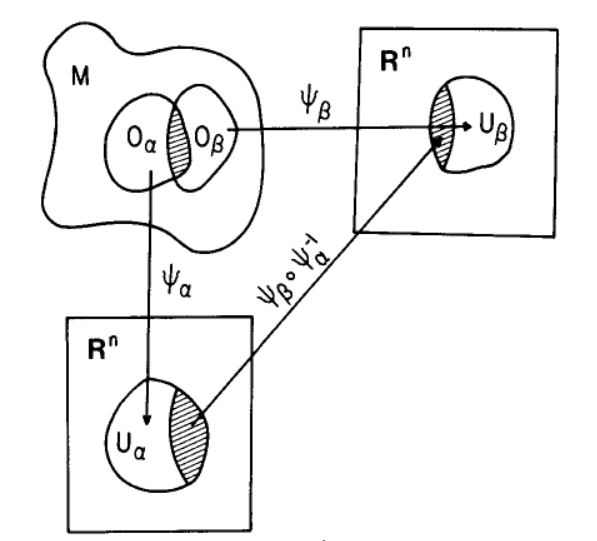
\includegraphics[scale=0.6]{manifold}
  \caption{An illustration of the map $\psi_\beta\circ\psi_\alpha^{-1}$ arising when two coordinate systems(Source: Wald\cite{wald})}
  \label{fig:manifold}
\end{figure}
Each map $\psi_\alpha$ is generally called a \textit{chart} by mathematicians and a \textit{coordinate system} by physicists.

\subsubsection*{Transformation of coordinates}
\begin{definition}{\textbf{\textit{Contravariant vector}}}
A contravariant vector or contravariant tensor of rank (order) 1 is a set of 
quantities, written as $X^a$ in the $x^a$-coordinate system, associated with a point P, which transforms under a change of coordinates according to 
$$X^{'a} =\sum_{b=1}^n \left[\dfrac{\partial x^{'a}}{\partial x^b}\right]_pX^b$$
\end{definition}
From here on we are going to use the \href{https://en.wikipedia.org/wiki/Einstein_notation}{\textbf{Einstein Summation Convention}}. We rewrite it as
$$X^{'a} =\dfrac{\partial x^{'a}}{\partial x^b} X^b $$
The index a occurring on each side of this equation is said to be \textbf{free} and may 
take on separately any value from 1 to n. The index b on the right-hand side is 
repeated and hence there is an implied summation from 1 to n. A repeated 
index is called \textbf{bound} or \textbf{dummy} because it can be replaced by any other index not already in use.
\begin{definition}{\textbf{\textit{Covariant vector}}}
a covariant vector or covariant tensor of rank (order) 1 is a set of quantities, written $X^a$ in the $x^a$-coordinate system, associated with a point P, which transforms according to 
$$X^{'}_a =\sum_{b=1}^n\left[\dfrac{\partial x^{b}}{\partial x^{'a}}\right]_p X_b=\dfrac{\partial x^{b}}{\partial x^{'a}} X_b $$
\end{definition}

\begin{figure}[h]
    \centering
  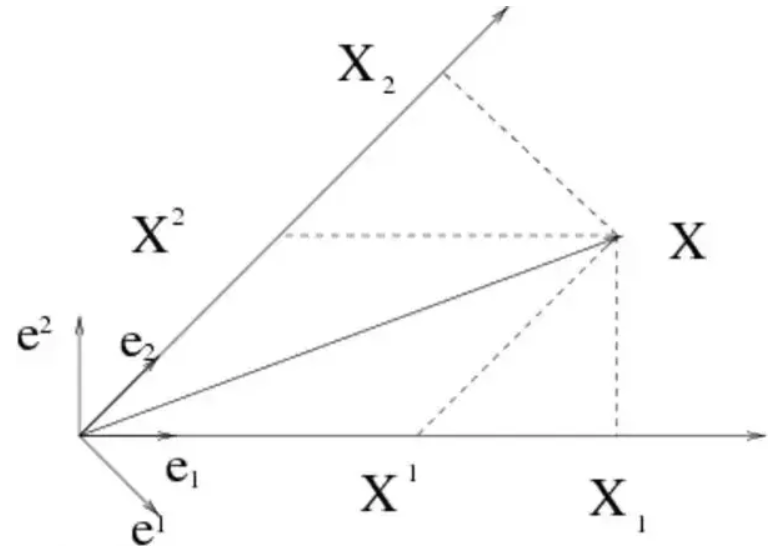
\includegraphics[scale=0.6]{vectors}
  \caption{An intuitive representation of both type of vectors}
  \label{fig:vectors}
\end{figure}

Position vectors etc are contravariant and vectors which is a gradient of a potential field etc. are covariant vectors.Also contravariant indices are given above and covariant indices below(see fig 3.2). The vectors are named as this because when you scale the units by a factor the contravariant vectors \textbf{contra-vary}(reduce by that factor) and covariant vectors \textbf{co-vary}.

A vector is an array containing elements which transforms in certain ways. We can generalise vectors and define \textbf{Tensors} which are multidimensional array transform in a similar way. A mixed tensor having contravariant rank p and covariant rank q is said to have type or valence (p, q). Such a vector transforms as-$$\tensor{X}{^{'i_1i_2\cdots i_p}_{j_1j_2\cdots j_q }}=\dfrac{\partial x^{'i_1}}{\partial x^{k_1}}\cdots \dfrac{\partial x^{'i_p}}{\partial x^{k_p}} \dfrac{\partial x^{l_1}}{\partial x^{'j_1}}\cdots \dfrac{\partial x^{l_q}}{\partial x^{'j_q}}  \tensor{X}{^{i_1i_2\cdots i_p}_{j_1j_2\cdots j_q }} $$

Suppose we find in one coordinate system that two tensors, $X^a_b=Y^a_b$ then by multiplying on both sides by $\dfrac{\partial x^{'c}}{\partial x^a}\dfrac{\partial x^b}{\partial x^{'d}} $ we get-
$$\dfrac{\partial x^{'c}}{\partial x^a}\dfrac{\partial x^b}{\partial x^{'d}} X^a_b =\dfrac{\partial x^{'c}}{\partial x^a}\dfrac{\partial x^b}{\partial x^{'d}}Y^a_b $$

$$\Rightarrow X^{'c}_{d}=Y^{'c}_{d}$$
Similarly we can say that all \textbf{tensorial equations are coordinate-independent}. We can add 2 \textbf{tensor fields} at a point to get a different tensor field. But we \textbf{cannot} add tensors at 2 different points to obtain a new tensor because the addition(or subtraction) does not follow the transformation rules(since the transformation matrix is calculated at 2 different points). However, under linear coordinate transformations they are tensors as the transformation matrix will be constant. 
A \textbf{totally symmetrical covariant tensor} is a covariant tensor  which is equal to its symmetric part.The symmetric part of $X_{a_1a_2\cdots a_r} $ is written as $X_{(a_1a_2\cdots a_r)}$ and is defined as
$$X_{(a_1a_2\cdots a_r)} =\dfrac{1}{r!}\text{(sum over all permutations of the indices $a_1$ to $a_r$)}$$
A \textbf{totally anti-symmetric tensor} is a covariant tensor  which is equal to its anti-symmetric part.The anti-symmetric part of $X_{a_1a_2\cdots a_r}$ is written as $X_{[a_1a_2\cdots a_r]} $ and is defined as
$$X_{[a_1a_2\cdots a_r]} =\dfrac{1}{r!}\text{(alternating sum over all permutations of the indices $a_1$ to $a_r$)}$$
For example,
$$X_{[abc]}=\dfrac{1}{6}(X_{abc}+X_{cab}+X_{bca}-X_{acb}-X_{cba}-X_{bac}) $$
We can multiply two tensors of type ($p_1$,$q_1$) and ($p_2$,$q_2$) together and obtain a tensor of type ($p_1$ + $p_2$, $q_1$ + $q_2$).

Given a tensor of mixed type (p, q), we can form a 
tensor of type (p — 1, q — 1) by the process of \textbf{contraction}, which simply involves setting a raised and lowered index equal. And it can be considered as a multiplication with \textbf{Kronecker tensor} . For example-
$$\delta^b_aX^a_{bcd}=X^a_{acd}=Y_{cd}$$

\begin{definition}{\textbf{\textit{Commutator or Lie bracket}}}
Given two vector fields X and Y we can define a new vector field called the 
commutator or Lie bracket of X and Y by 

$$[X, Y]=XY-YX $$
It follows from the above equation that
$$[X, Y]=-[Y, X] $$
$$[X, [Y, Z]]+[Y, [Z, X]]+[Z, [X, Y]]=0\text{ (Jacobi's identity)}  $$
\end{definition}
We can also interpret a vector field as an operator defined as-(here $\partial_a=\dfrac{\partial}{\partial x^a}$)
$$X=X^a\partial_a $$
The above interpretation is coordinate independent(i.e $X^{'a}\partial^{'}_{a} = X^a\partial_a $). Coordinate free approach can be done more generally and can be applied but in this article we are not using it.

In any coordinate system, we may think of the quantities $\left[\dfrac{\partial}{\partial x^a}\right]_P$ as 
forming a basis for all the vectors at P, since any vector at P is given by $$X=[X^a]_p[\partial_a]_p $$. The vector space of all the 
contravariant vectors at P is known as the tangent space at P and is written 
$T_P(M)$. In general, the tangent space at any point in a manifold is different from the underlying manifold. In Euclidean space and Minkowski space-time the tangent space at each point coincides with the manifold.

\subsection{Tensor calculus}
We denote a partial derivative of a contravariant vector as $\partial_bX^a$ or  $\dfrac{\partial}{\partial x^b}X^a$ or $X^a_{ ,b}$ or $X^a_{ |b}$. These partial derivatives do not transform the way vectors do. This is true for tensors in general. So we have to define other types of differentiation  which retain the \textbf{tensorial character}. We might think of defining differentiation as the subtraction of two very nearby points devided by some small quantity like distance. But again in general the \textbf{the difference of tensors at different points need not be a tensor}.
\subsubsection{The Lie derivative}
This is a derivative of a tensor field using another vector field. Let $Y(x)$ be a vector field. We now use the vector field $Y(x)$ to provide a congruence of curves along which derivatives of a tensor are calculated. Intuitively we are going to drag the tensor at some point P along the curve passing through P to some neighbouring point Q, and then compare this 'dragged-along tensor' with the tensor already there. Since the dragged-along tensor will be of the same type as the tensor already at Q, we can subtract the two tensors at Q and so define a derivative by some limiting process as Q tends to P. The curve $x^a(u)$ passing through P is
$$\dfrac{dx^a}{du}=X^a(x(u))$$
Transforming using
$$x^{'a}=x^a+\delta uX^a(x)=x^a+\delta x^a$$
Then we define Lie derivative of $\tensor{T}{^{i_1i_2\cdots i_p}_{j_1j_2\cdots j_q }}$ denoted by $L_X \tensor{T}{^{i_1i_2\cdots i_p}_{j_1j_2\cdots j_q }}$ as
$$L_X \tensor{T}{^{i_1i_2\cdots i_p}_{j_1j_2\cdots j_q }}=\lim_{\delta u\to 0} \dfrac{\tensor{T}{^{i_1i_2\cdots i_p}_{j_1j_2\cdots j_q }}(x')-\tensor{T}{^{'i_1i_2\cdots i_p}_{j_1j_2\cdots j_q }}(x')}{\delta u}$$
From the above equation we can deduce that-
\begin{multline*}
L_X \tensor{T}{^{i_1i_2\cdots i_p}_{j_1j_2\cdots j_q}} =Y^c(\partial_c\tensor{T}{^{i_1i_2\cdots i_p}_{j_1j_2\cdots j_q }})\\-(\partial_c Y^{i_1})\tensor{T}{^{ci_2\cdots i_p}_{j_1j_2\cdots j_q}}-\cdots- (\partial_c Y^{i_p})\tensor{T}{^{i_1i_2\cdots c}_{j_1j_2\cdots j_q}}\\+(\partial_c Y^{j_1})\tensor{T}{^{i_1i_2\cdots i_p}_{cj_2\cdots j_q}}+ \cdots +(\partial_c Y^{j_q})\tensor{T}{^{i_1i_2\cdots i_p}_{j_1j_2\cdots c}}
\end{multline*}
\begin{itemize}
    \item It is linear.
    \item It is Leibniz; that is, it satisfies the usual product rule for differentiation.
    \item the Lie derivative of a tensor of type (p, q) is again a tensor of type (p, q).
    \item It commutes with contraction
    \item The Lie derivative of a contravariant vector field $Y^a$ is given by the Lie bracket of $X$ and $Y$.
\end{itemize}

\subsubsection{Covariant Differentiation}
Let us first consider a general contravariant vector$\textbf{V}$ expressed in $e_a0 $ is given by $\textbf{V}=V^ae_a$. The derivative of it is-
$$\dfrac{\partial \textbf{V}}{\partial x^b}=\dfrac{\partial v^a}{\partial x^b}\textbf{e}_a+ V^a\dfrac{\partial\textbf{e}_a}{\partial x^b}$$
The change in a basis vector is itself a vector, so it can be written in terms
of the original set of basis vectors-
$$\dfrac{\partial\textbf{e}_a}{\partial x^b}=\Gamma^c_{ab}\textbf{e}_c$$
it follows after inter changing the dummy indices-
$$\dfrac{\partial \textbf{V}}{\partial x^b}=\dfrac{\partial v^a}{\partial x^b}\textbf{e}_a+V^c\Gamma^a_{cb}\textbf{e}_a$$
We denote the above equation as
$$\nabla_bV^a=V^a_{;b}=\dfrac{\partial v^a}{\partial x^b}+V^c\Gamma^a_{cb} $$
where the $\Gamma^a_{cb}$ are defined by this equation, and are called the \textbf{connections} or \textbf{affine connections} (they are not tensors).

By using the condition that the covariant derivative is a tensor we get the following transformation properties for the affline connections(both are equivalent).
$$\Gamma^{'a}_{bc}=\dfrac{\partial x^{'a}}{\partial x^d}\dfrac{\partial x^{e}}{\partial x^{'b}}\dfrac{\partial x^{f}}{\partial x^{'c}}\Gamma^{d}_{ef}-\dfrac{\partial x^{d}}{\partial x^{'c}}\dfrac{\partial x^{e}}{\partial x^{'b}}\dfrac{\partial^2 x^{'a}}{\partial x^e \partial x^f} $$
$$\Gamma^{'a}_{bc}=\dfrac{\partial x^{'a}}{\partial x^d}\dfrac{\partial x^{e}}{\partial x^{'b}}\dfrac{\partial x^{f}}{\partial x^{'c}}\Gamma^{d}_{ef}+ \dfrac{\partial x^{'a}}{\partial x^{f}}\dfrac{\partial^2 x^f}{\partial x^{'b} \partial x^{'c}} $$
For a general tensor we can generalize the covariant derivative by using that it should be Leibniz etc. The generalized formula is given by-
\begin{multline*}
\nabla_e \tensor{T}{^{i_1i_2\cdots i_p}_{j_1j_2\cdots j_q}} =\partial_e\tensor{T}{^{i_1i_2\cdots i_p}_{j_1j_2\cdots j_q }}\\
+\tensor{T}{^{fi_2\cdots i_p}_{j_1j_2\cdots j_q }}\Gamma^{i_1}_{fe}+\cdots+\tensor{T}{^{i_1i_2\cdots f}_{j_1j_2\cdots j_q }}\Gamma^{i_p}_{fe}\\-\tensor{T}{^{i_1i_2\cdots i_p}_{fj_2\cdots j_q}}\Gamma^{f}_{j_1e}-\cdots-\tensor{T}{^{i_1i_2\cdots i_p}_{j_1j_2\cdots f}}\Gamma^{f}_{j_qe}
\end{multline*}
\begin{itemize}
    \item The name covariant derivative is due to the fact that the derivative of a tensor of type (p, q) is of type (p, q+1)
    \item It commutes with contraction
    \item It is Leibniz.
    \item It is linear
    \item It is not commutative.
    \item We define $\Bar{\delta}^a(x)=-\Gamma^a_{bc}X^b(x)\delta x^c$ and the vector $X^a(x)+\Bar{\delta}X^a(x)$ is said to be parallel to $X^a$.
\end{itemize}
It follows directly from the transformation laws that the sum of two 
connections is \textbf{not} a connection or a tensor. However, the difference of two connections is a tensor of valence (1,2), because the inhomogeneous term cancels out in the transformation. For the same reason, the anti-symmetric part of a $\Gamma^a_{bc} $, namely,
$$\tensor{T}{^a_{bc}}=\Gamma^a_{bc}-\Gamma^a_{cb} $$
is a tensor called the \textbf{torsion tensor}. If the torsion tensor vanishes, then the 
connection is symmetric, i.e.
$$\Gamma^a_{bc}=\Gamma^a_{cb} $$
From now on, unless we state otherwise, we shall restrict ourselves to 
symmetric connections, in which case the torsion vanishes.The assumption 
that the connection is symmetric leads to the following useful result. In the 
expression for a Lie derivative of a tensor, all occurrences of the \textbf{partial derivatives} may be replaced by \textbf{covariant derivatives}.

\subsubsection{Absolute Derivative}
In Euclidean spaces we know how to transport vectors parallel to themselves. There we transport a vector along a curve C given by $x=x(u)$ with tangent field $\frac{dx^a}{dx}=X^a$ as follows- we assume a vector field such that $\dfrac{dv^a}{du}=0$ along the curve. Now we ca generalize in to any tensor as follows. We define \textbf{Absolute Derivative} denoted by $\dfrac{D}{Du}(\tensor{T}{^{i_1i_2\cdots i_p}_{j_1j_2\cdots j_q}})$ or $\nabla_X \tensor{T}{^{i_1i_2\cdots i_p}_{j_1j_2\cdots j_q}}$ as follows-
$$\dfrac{D}{Du}(\tensor{T}{^{i_1i_2\cdots i_p}_{j_1j_2\cdots j_q}})=\nabla_X \tensor{T}{^{i_1i_2\cdots i_p}_{j_1j_2\cdots j_q}}=X^c\nabla_c \tensor{T}{^{i_1i_2\cdots i_p}_{j_1j_2\cdots j_q}}$$
The tensor is said to be \textbf{parallely propagated} or \textbf{transported} along the curve C if 
$$\dfrac{D}{Du}(\tensor{T}{^{i_1i_2\cdots i_p}_{j_1j_2\cdots j_q}})=0$$

\begin{itemize}
    \item $\nabla_{fX+gY}T=f\nabla_XT+g\nabla_YT$(here f,g are smooth functions)
\end{itemize}
\begin{definition}{\textbf{\textit{Affine Geodesic}}}
It is defined as a curve along which the tangent vector is propagated parallel to itself. In other words, the parallely propagated vector at any point of the curve is is, parallel or proportional, to the tangent vector at that point-
$$\dfrac{D}{Du}(\dfrac{dx^a}{du})=\lambda(u)\dfrac{dx^a}{du}$$
or
$$\nabla_X X^a=\lambda X^a $$
which on solving gives
$$\dfrac{d^2x^a}{du^2}+\Gamma^a_{bc}\dfrac{dx^b}{du}\dfrac{dx^c}{du}=\lambda\dfrac{dx^a}{du} $$

\end{definition}
If the curve is parametrized in such a way that $\lambda$ vanishes, then the  
parameter is a privileged parameter called an \textbf{affine parameter}, often  
conventionally denoted by $s$, and the affine geodesic equation reduces to $\nabla_X X^a=0$ or 
$$\dfrac{d^2x^a}{ds^2}+\Gamma^a_{bc}\dfrac{dx^b}{ds}\dfrac{dx^c}{ds}=0 $$.
An affine parameter s is only defined up to an \textbf{affine transformation}-$s\rightarrow\alpha s+\beta$($\alpha$and $\beta$ are constants)
We can use the affine parameter s to define the \textbf{affine length} of the geodesic between two points $P_1$ and $P_2$ by $\int_{P_1}^{P_2}$, and so 
we can compare lengths on the \textbf{same geodesic}(to compare lengths on different geodesics we need a metric). Corresponding to every direction at a point there is a unique geodesic passing through the point.
\subsubsection*{Riemann Tensor}
As covariant differentiation is not commutative we define commutator as
$$\nabla_{[c}\nabla_{d]} \tensor{T}{^{i_1i_2\cdots i_p}_{j_1j_2\cdots j_q}}=\nabla_c\nabla_d \tensor{T}{^{i_1i_2\cdots i_p}_{j_1j_2\cdots j_q}}-\nabla_d\nabla_c \tensor{T}{^{i_1i_2\cdots i_p}_{j_1j_2\cdots j_q}} $$
If we work out the commutator in the case of a vector $X^a$. We will get
$$\nabla_{[c}\nabla_{d]} X^a=(\partial_c\Gamma^a_{bd}-\partial_d\Gamma^a_{bc}+\Gamma^e_{bd}\Gamma^a_{ec}-\Gamma^e_{bc}\Gamma^a_{ed})X^b+(\Gamma^e_{cd}-\Gamma^e_{dc})\nabla_e X^a $$
We can reduce it to the below equation-
$$\nabla_{[c}\nabla_{d]} X^a=\tensor{R}{^{a}_{bcd}}X^b+(\Gamma^e_{cd}-\Gamma^e_{dc})\nabla_e X^a $$
by defining $\tensor{R}{^{a}_{bcd}}$ (called as the Riemann tensor) as-
$$\tensor{R}{^{a}_{bcd}}=\partial_c\Gamma^a_{bd}-\partial_d\Gamma^a_{bc}+\Gamma^e_{bd}\Gamma^a_{ec}-\Gamma^e_{bc}\Gamma^a_{ed} $$


At any point P in a manifold, we can introduce a special coordinate system, called a \textbf{geodesic coordinate system}, in which $[\Gamma^a_{bc}]_P=0$
It can be shown that the result can be extended to obtain a 
coordinate system in which the connection vanishes along a curve, but not in 
general over the whole manifold. If, however, there exists a special coordinate 
system in which the connection vanishes everywhere, then the manifold is 
called \textbf{affine flat} or simply \textbf{flat}.

If, we can transport a vector from one point to any other and the resulting vector is independent of the path taken, then the connection is called \textbf{integrable}. We can prove following lemmas-
\begin{lemma}
A necessary and sufficient condition for a connection to be integrable is that the Riemann tensor vanishes.
\end{lemma}
\begin{lemma}
A necessary and sufficient condition for a manifold to be affline flat is that the connection is symmetric and integrable.
\end{lemma}
By combining above 2 we get-
\begin{theorem}[]
A necessary and sufficient condition for a manifold to be affline flat is that the \textbf{Riemann tensor vanishes}. 
\end{theorem}
\subsubsection*{The Metric}
In Euclidean spaces we know that $(ds)^2=(dx^a)^2$.We can generalise this notion using a \textbf{metric} Any symmetric covariant tensor field of rank 2, say $g_{ab}(x)$, defines a metric. A manifold with a metric is called a \textbf{Riemannian manifold}. The infinitesimal distance or interval between two  neighbouring points $x^a$ and $x^a + dx^a$ is defined by
$$ds^2=(ds)^2=g_{ab}(x)dx^adx^b $$
the length or norm of a contravariant vector $X^a$ is defined by
$$X^2=g_{ab}(x)X^aX^b $$
The metric is said to be \textbf{positive definite} or \textbf{negative definite} if, for all vectors 
$X$, $X^2$ > 0 or $X^2$ < 0, respectively. Otherwise, the metric is called indefinite(ex-spacetime in relativity).
The angle between two vectors $X^a$ and $Y^a$ with $X^2\neq0$ and $Y^2\neq0$ is given by 
$$cos(X,Y)=\dfrac{g_{ab}X^aY^b}{\sqrt{|X^2|}\sqrt{|Y^2|}} $$
If the metric is indefinite then there exist vectors which are orthogonal to themselves called \textbf{null vectors}.
The determinant of the metric is denoted by $g=\text{det}(g_{ab})$.
If it is non zero then its inverse is called as \textbf{contravariant metric} denoted by $g^{ab}$. We use $g_{ab}$,$g^{ab}$ to lower and raise the indices.

From now we will be working with Riemannian manifolds , we shall regard such 
associated contravariant and covariant tensors as representations of the 
same geometric object. In particular,$g_{ab}$, $\delta^b_a$ and $g^{ab}$ may all be thought of as different representations of the metric $g$.

The interval S between two points $P_1$ and $P_2$ on a timelike curve $C$ given by $x=x^a(u)$ is given by
$$s=\int^{P_2}_{P_1}\dfrac{ds}{du}du=\int^{P_2}_{P_1}\sqrt{g_{ab}\dfrac{dx^a}{du}\dfrac{dx^b}{du}} du$$
We define a \textbf{timelike metric geodesic} between any two points $P_1$ and $P_2$ as the privileged curve joining them whose interval is stationary under small variations that vanish at the end points. Using calculus of variations, we solve it the next chapter. The solution is(the equation of geodesics)-
$$g_{ab}\dfrac{d^2x^b}{du^2}+\{bc,a\}\dfrac{dx^b}{du}\dfrac{dx^c}{du}=\left(\dfrac{\frac{d^2s}{du^2}}{\frac{ds}{du}}\right)\dfrac{dx^b}{du} $$
where $\{ab,c\} $ is called the Christoffel symbol of 
the first kind and is defined by
$$\{ab,c\}=\frac{1}{2}(\partial_bg_{ac}+\partial_ag_{bc}-\partial_cg_{ab})$$
Multiplying the solution by $g^{ad}$ we get the simplified form
$$\dfrac{d^2x^a}{du^2}+\begin{Bmatrix}a\\bc\end{Bmatrix} \dfrac{dx^b}{du}\dfrac{dx^c}{du}=\left(\dfrac{\frac{d^2s}{du^2}}{\frac{ds}{du}}\right)\dfrac{dx^b}{du}$$
where $\begin{Bmatrix}a\\bc\end{Bmatrix}$ is called the Christoffel symbol of 
the second kind and is defined by
$$\stirling{a}{bc}=g^{ad}\{bc,d\} $$
If, we choose a parameter u which is linearly related to the interval s then the right-hand side vanishes. In the case of an indefinite metric, there exist geodesics for which the distance between any two points is zero called \textbf{null geodesics}. It can be shown that these curves can be parametrized by a special parameter u, called an \textbf{affline parameter}, such that their equation does not possess a right-hand side,that is-
$$\dfrac{d^2x^a}{du^2}+\begin{Bmatrix}a\\bc\end{Bmatrix} \dfrac{dx^b}{du}\dfrac{dx^c}{du}=0 $$

\subsubsection*{The Metric connection}
If we have a manifold endowed with both an affine connection and 
metric, then it possesses two classes of curves, \textbf{affine geodesics} and \textbf{metric geodesics}, which will be different. However the two classes will coincide if we take
$$\Gamma^a_{bc}=\stirling{a}{bc}$$
$$\Rightarrow \Gamma^a_{bc}=\frac{1}{2}g^{ad}(\partial_bg_{dc}+\partial_cg_{db}-\partial_dg_{bc})$$
From now on, we shall always work with the metric connection and we shall denote it by $\Gamma^a_{bc}$ rather than $\stirling{a}{bc}$, 
\begin{theorem}[]
 If $\nabla_a$ denotes covariant derivative with respect to the affine 
connection $\Gamma^a_{bc}$, then the necessary and sufficient condition for the covariant derivative of the metric to vanish is that the connection is the metric connection.
\end{theorem}
In a metric connection-
\begin{itemize}
\item $\nabla_c\delta^a_b=0$
\item $\nabla_cg{^ab}=0$
\item $\partial_cg_{ab}=\Gamma^d_{ac}g_{db}+\Gamma^d_{bc}g_{ad}$
\item $\partial_c g=g g^{ab}\partial_cg_{ab}=2g\Gamma^a_{ac}$
\item $\nabla_c g=0 $
\end{itemize}
If, there does exist a coordinate system in which the metric reduces to diagonal form with $\pm 1$ diagonal elements everywhere, then the metric is called \textbf{flat}.
\begin{theorem}[]
A necessary and sufficient condition for a metric to be flat is that its Riemann tensor vanishes.
\end{theorem}
\subsubsection*{Tensors related to the Riemann tensor}
We know that
$$\tensor{R}{^{a}_{bcd}}=\partial_c\Gamma^a_{bd}-\partial_d\Gamma^a_{bc}+\Gamma^e_{bd}\Gamma^a_{ec}-\Gamma^e_{bc}\Gamma^a_{ed} $$
$$\Gamma^a_{bc}=\frac{1}{2}g^{ad}(\partial_bg_{dc}+\partial_cg_{db}-\partial_dg_{bc})$$
We get the following symmetries-
$$\tensor{R}{^{a}_{bcd}}=-\tensor{R}{^{a}_{bdc}} $$
$$\tensor{R}{^{a}_{bcd}}+\tensor{R}{^{a}_{dbc}}+\tensor{R}{^{a}_{cdb}}=0 $$
$$\tensor{R}{_{abcd}}=-\tensor{R}{_{abdc}}=-\tensor{R}{_{bacd}}=\tensor{R}{_{cdab}} $$
$$\tensor{R}{_{abcd}}+\tensor{R}{_{adbc}}+\tensor{R}{_{acdb}}= 0$$
where $\tensor{R}{_{abcd}}=g_{ae}\tensor{R}{^{e}_{bcd}}$
In n-dimensions the number of independent components in $\tensor{R}{^{a}_{bcd}}$ is $\dfrac{n^2(n^2-1)}{12}$
The curvature tensor satisfies a set of differential identities called the \textbf{Bianchi identities}:
$$\nabla_a \tensor{R}{_{debc}}+\nabla_c \tensor{R}{_{deab}}+\nabla_b \tensor{R}{_{deca}}=0 $$
The \textbf{Ricci tensor} is defined by the contraction
$$\tensor{R}{_{ab}}=\tensor{R}{^{c}_{acb}}=g^{cd}\tensor{R}{_{dacb}} $$
The \textbf{Ricci scalar} or \textbf{curvature scalar} is defined by the contraction
$$R=g^{ab}\tensor{R}{_{ab}}$$
These two can be used to define the \textbf{Einstein tensor}-
$$G_{ab}=\tensor{R}{_{ab}}-\frac{1}{2}g_{ab}R $$
The Einstein tensor can be shown to 
satisfy the \textbf{contracted Bianchi identities}-
$$\nabla_b \tensor{G}{_{a}^b} $$
If n = 4, $\tensor{R}{_{abcd}}$ has twenty independent components — ten of which are given by Rab and the remaining ten by the \textbf{Weyl tensor}. 
The Weyl tensor or conformal tensor $\tensor{C}{_{abcd}}$ is defined in n dimensions, ($n>2$) by
\begin{multline*}
\tensor{C}{_{abcd}} =\tensor{R}{_{abcd}}+\frac{1}{n-2}(g_{ab}\tensor{R}{_{cb}}+g_{bc}\tensor{R}{_{da}}-g_{ac}\tensor{R}{_{db}}-g_{bd}\tensor{R}{_{ca}}) \\
+\frac{R}{(n-1)(n-2)}(g_{ac}g_{db}-g_{ad}g_{cb})\\
\end{multline*}
In 4-d
\begin{multline*}
\tensor{C}{_{abcd}} =\tensor{R}{_{abcd}}+\frac{1}{2}(g_{ab}\tensor{R}{_{cb}}+g_{bc}\tensor{R}{_{da}}-g_{ac}\tensor{R}{_{db}}-g_{bd}\tensor{R}{_{ca}}) \\
+\frac{R}{6}(g_{ac}g_{db}-g_{ad}g_{cb})\\
\end{multline*}
Weyl tensor possesses the all symmetries as the Riemann tensor, it possesses an additional symmetry $\tensor{C}{^a_{bcd}}=0 $. One can think of the Weyl tensor as that part of the curvature tensor for which all contractions vanish.

Two metrics $g_{ab}$ and $\overline{g}_{ab}$ are said to be \textbf{conformally related} or \textbf{conformal} to each other if $\overline{g}_{ab}=\Omega^2 g_{ab} $ where $\Omega(x)$ is a non-zero differentiable function. Given a manifold with two metrics defined on it which are conformal, then it is straightforward to show that angles between vectors and ratios of magnitudes 
of vectors, but not lengths, are the same for each metric. The metrics also possess the same Weyl tensor(it is \textbf{conformally invariant} but $g_{ab}$,$\Gamma^a_{bc}$,$\tensor{R}{^a_{bcd}}$  are not). A metric is said to be \textbf{conformally flat} if it can be reduced to the form $g_{ab}=\Omega^2 \eta_{ab} $ where $\eta_{ab}$ is a flat metric. We can prove-
\begin{theorem}[]
A necessary and sufficient condition for a metric to be conformally fiat is that its Weyl tensor vanishes everywhere. 
\end{theorem}
\begin{theorem}[]
Any two dimensional Riemannian manifold is conformally flat.
\end{theorem}


\subsection{Integration,variation and symmetry}
\subsubsection*{Tensor densities}
A tensor density of weight W, denoted conventionally by a gothic letter, 
$\tensor{\mathfrak{T}}{^{i_1\cdots}_{j_1\cdots}}$, transforms like an ordinary tensor, except that in addition the Wth 
power of the Jacobian $J=\left|\dfrac{\partial x^a}{\partial x^{'a}}\right|$ appears as a factor, i.e.
$$\tensor{\mathfrak{T}}{^{'i_1\cdots}_{j_1\cdots}}=J^w\dfrac{\partial x^{'i_1}}{\partial x^{k_1}}\cdots\dfrac{\partial x^{l_1}}{\partial x^{'j_1}}\cdots \tensor{\mathfrak{T}}{^{k_1\cdots}_{l_1\cdots}}$$
The product of two tensor densities of weight $W_1$ and $W_2$ is a tensor 
density of weight $W_1+W_2$. We defie its covariant derivative as
$$\nabla_c\tensor{\mathfrak{T}}{^{i_1\cdots}_{j_1\cdots}}=\text{usual terms if }\tensor{\mathfrak{T}}{^{i_1\cdots}_{j_1\cdots}}\text{ were a tensor}-W\Gamma^d_{dc}\tensor{\mathfrak{T}}{^{i_1\cdots}_{j_1\cdots}} $$
the covariant derivative of a vector density of weight W i
$$\nabla_c\tensor{\mathfrak{T}}{^{a}}=\partial_c\tensor{\mathfrak{T}}{^{a}}+\Gamma^a_{bc}\tensor{\mathfrak{T}}{^{b}}-W\Gamma^b_{bc}\tensor{\mathfrak{T}}{^{a}} $$
In the special case when W = +1 and $c=a$, we get the important result (both these quantities are scalar densities of weight 1)
$$ \nabla_a\tensor{\mathfrak{T}}{^{a}}=\partial_a\tensor{\mathfrak{T}}{^{a}}$$

\subsubsection*{The Levi-Civita alternating symbol}
The Levi-Civita alternating symbol(it is similar to Kronecker delta) $\epsilon^{abcd}$  is a completely anti-symmetric tensor density of weight +1 and contravariant rank 4, whose values in any coordinate system is +1 or — 1 if, abcd is an even or odd permutation of 0123, respectively, and zero otherwise.
It can be used, in particular, to form the determinant of a second-rank density
$$\text{det}\tensor{\mathfrak{T}}{^{ab}}=\frac{1}{4!}\epsilon_{abcd}\epsilon_{efgh}\tensor{\mathfrak{T}}{^{ae}}\tensor{\mathfrak{T}}{^{bf}}\tensor{\mathfrak{T}}{^{cg}}\tensor{\mathfrak{T}}{^{dh}} $$
We define the generalized Kronecker delta by 
$$\delta^{ab}_{cd} =\begin{vmatrix}
\delta^a_c & \delta^b_c \\
\delta^a_d  & \delta^b_d
\end{vmatrix}
$$
We can similarly generalize for $\delta^{abc}_{def}\cdots$. We also get
$$\epsilon^{abcd}\epsilon_{efgh}=\delta^{abcd}_{efgh}$$
$$\epsilon^{abcd}\epsilon_{efgd}=\delta^{abc}_{efg}$$
$$\epsilon^{abcd}\epsilon_{efcd}=2\delta^{ab}_{ef}$$
$$\epsilon^{abcd}\epsilon_{ebcd}=3!\delta^{a}_{e}$$
$$\epsilon^{abcd}\epsilon_{abcd}=4!$$
\subsubsection*{The metric determinant }
As $g_{ab}$ is (0,2) type tensor its determinat is a scalar density of weight +2. In the later chapters, we shall be working with metrics of negative signature in which case g will be negative, and so we write it the equivalent form
$$(-g^{'})=J^2(-g) $$
$$\sqrt{-g^{'}}=J(\sqrt{-g})$$
So $(-g)^{\frac{1}{2}}$ is a scalar density of weight +1. It will be useful in integration. We get
$$\nabla_a[(-g)^{\frac{1}{2}}\tensor{T}{^{i_1\cdots}_{j_1\cdots}}]=\partial_a[(-g)^{\frac{1}{2}}\tensor{T}{^{i_1\cdots}_{j_1\cdots}}]$$
$$\nabla_c(-g)^{\frac{1}{2}}=0 $$
$$\Rightarrow\nabla_a[(-g)^{\frac{1}{2}}\tensor{T}{^{i_1\cdots}_{j_1\cdots}}]=(-g)^{\frac{1}{2}}\nabla_a[\tensor{T}{^{i_1\cdots}_{j_1\cdots}}]$$
\subsubsection*{Integrals}
Unlike tensors in general, we can add a scalar field $\Phi$ evaluated at two 
different points,  and the resulting quantity is still a scalar. It turns out that the volume element $d\Omega$ is not a scalar but, as we shall see, a scalar density of weight $—1$. It follows that we can integrate a scalar density $\Phi$ of weight +1 over a region $\Omega$, 
$$\int_{\Omega}\Phi d\Omega $$
Consider an m-dimensional subspace of M whose parametric equation is $x^a=x^a(u^i)$. The volume element of this subspace is defined to be
$$d\tau^{a_1\cdots a_m}=\delta^{a_1\cdots a_m}_{b_1\cdots b_m}\dfrac{\partial x^{a_1}}{\partial u_1}\cdots\dfrac{\partial x^{a_m}}{\partial u_m}du^1\cdots du^m $$
This element is an mth rank contravariant tensor under coordinate  
transformations and behaves like a scalar under arbitrary change of parameter. 
Hence, if $X_{a_1\cdots a_m}$ is an mth rank covariant tensor, then $X_{a_1\cdots a_m}d\tau^{a_1\cdots a_m}$ is a scalar under both coordinate and parameter transformations, and we can form the integral.

\begin{theorem}[Stokes' theorem]
Stokes' theorem for a simply connected m-dimensional subspace $\Omega_m$ bounded by the (m - l)-dimensional subspace $\partial\Omega_m=\Omega_{m-1}$:
$$\int_{\partial\Omega_m}X_{a_1\cdots a_m}d\tau^{a_1\cdots a_{m-1}}=\int_{\Omega_m}\partial_{a_m} X_{a_1\cdots a_m}d\tau^{a_1\cdots a_m}$$

\end{theorem}
The Euler-Lagrange equation for $L$ is-
$$\dfrac{\partial L}{\partial y}-\dfrac{d}{dx}\left(\dfrac{\partial L}{\partial y'}\right) $$
From the above equation we can prove the geodesic equation-
$$g_{ab}\dfrac{d^2x^b}{du^2}+\{bc,a\}\dfrac{dx^b}{du}\dfrac{dx^c}{du}=\left(\dfrac{\frac{d^2s}{du^2}}{\frac{ds}{du}}\right)\dfrac{dx^b}{du} $$

A metric gab is \textbf{form-invariant} or simply \textbf{invariant} under the
transformation $x^a\rightarrow x^{'a}$ if $g'_{ab}(y)=g_{ab}(y)$ for all coordinates $y^c$. Then a transformation leaving gab form-invariant is called an \textbf{isometry}. \textbf{Killing vector fields} are those which satisfy $L_{X}g_{ab}=0$ .It can be shown that
\begin{lemma}An infinitesimal isometry is generated by a Killing vector $X^a(x)$ satisfying $L_{X}g_{ab}=0$.
\end{lemma}
\subsection{Special Relativity using Minkowski space-time}
Special Relativity gave us the notion of \textbf{spacetime}, which is a \textbf{geometrical representation} of space and time in a 4-d space.
The standard convention here is that the Greek alphabet($\mu$,$\nu$ etc) is used for \textbf{space and time} components where as the Latin alphabet($i$,$j$ etc) is used for only \textbf{spatial components}. From here on we take $c=1$ for \textbf{convenience}.
\textbf{Minkowski space-time}, or simply \textbf{flat space}, is defined as a  
four-dimensional manifold endowed with a flat metric of signature - 2. Since the metric is flat, there exists a special coordinate system covering the whole manifold in which the metric is diagonal, with diagonal elements equal to $\pm$ 1. The special coordinate system is called a 
\textbf{Minkowski coordinate system} and is written 

\begin{equation}
    (x^a)=(ct,x,y,z)=(t,x,y,z)
\end{equation}
We use the \textbf{timelike sign convention} or \textbf{Landau–Lifshitz sign convention} in which the Minkowski line element takes the form
\begin{equation}
ds^2=dt^2-dx^2-dy^2-dz^2=\eta_{ab}dx^adx^b
\end{equation}
where $\eta_{ab}=\text{diag}(1,-1,-1,-1)$ is called the \textbf{Minkowski metric}. Its Riemann curvature tensor is zero as the metric is constant. But the Riemann tensor vanishes for any coordinate system.(Example in spherical coordinates $g_{ab}=\text{diag}(1,-1,-r^2-r^2sin^2\theta)$).
If $X$ is a vector then it is said to be
\begin{itemize}
    \item timelike if $X^2>0$
    \item lightlike or null if $X^2=0$
    \item spacelike if $X^2<0$
\end{itemize}
The set of all lightlike points is called \textbf{null cone} or \textbf{light cone}(It is the equation of a double cone). This null cone lies in the tangent space $T_P$ at $P$, but since it is easy to show that the tangent space is itself a Minkowski manifold we can identify the tangent space with the 
underlying manifold and regard the null cone as lying in the manifold. We 
will \textbf{not} be able to do this when we go on to consider non-flat manifolds. manifolds. If we define the timelike vector $T^a$ in Minkowski coordinates by  $T^a = (1, 0, 0, 0)$, then a timelike or null vector $X^a$ is said to be
\begin{itemize}
    \item future pointing  if $\eta_{ab}X^aT^b>0$(it will be in furture cone)
    \item past pointing  if $\eta_{ab}X^aT^b<0$(it will be in past cone)
\end{itemize}
The \textbf{Lorentz transformations} are defined as those linear homogeneous  
transformations of Minkowski coordinates which leave the Minkowski metric $\eta_{ab}$ invariant.

\begin{equation}
    x^{'a}=\tensor{L}{^a_b}x^b
\end{equation}

or

$$\tensor{L}{^a_b}=\dfrac{\partial x^{'a}}{\partial x^b} $$
It follows form previous result that
\begin{equation}
  \tensor{L}{^a_c}\tensor{L}{^b_d}\eta_{ab}=\eta_{cd}  
\end{equation}
As Lorentz transformations are isometries it follows that Lorentz 
transformations preserve lengths and innner products of vectors. The Lorentz 
transformations form a group called the \textbf{Lorentz group L}.
The matrix $\tensor{L}{^a_b}$ is invertible, because if we take determinants of each side of (3.4) we get det($\tensor{L}{^a_b} $)$=\pm1$. We get by keeping c=d=0
$$(\tensor{L}{^0_0})^2-[(\tensor{L}{^1_0})^2+(\tensor{L}{^2_0})^2+(\tensor{L}{^3_0})^2]=1 $$
If det($\tensor{L}{^a_b}$) = +1, then it is called proper or orientation preserving.
If $\tensor{L}{^0_0} > 1$, then$\tensor{L}{^a_b} $ is called orthocronous or 
time-orientation preserving.
The proper orthochronous transformations, denoted by $\tensor{L}{^\uparrow_+}$ (read 'L arrow plus') from a subgroup of L.
The \textbf{Poincare group} P consists of those linear inhomogeneous  
transformations which leave $\eta_{ab}$ invariant. A Poincare transformation is made up of a Lorentz transformation together with an arbitrary translation (in space and time), i.e.
$$x^{'a}=\tensor{L}{^a_b}x^b+t^a $$
A \textbf{timelike world-line} or \textbf{timelike curve} is defined as a curve whose tangent vector is everywhere timelike. If, in particular, the curve is a geodesic, it is called a \textbf{timelike geodesic}. Timelike curves represent tracks on which material particles or observers can travel. Everything in upcone is called the future and in the downcone is called past. The remaining space do not have any fixed temporal order (it depends on the frame).
Since $\Gamma^a_{bc}$ vanishes in Minkowski coordinates, the equations for a non-null geodesic reduce to
\begin{equation}
    \dfrac{d^2x^a}{du^2}=0
\end{equation}
for some affine parameter u, where the tangent vector satisfies 
$$\eta_{ab}\dfrac{dx^a}{du}\dfrac{dx^b}{du}=k $$
The geodesic is timelike or spacelike depending on whether $k>0$ or $k<0$, 
respectively. In the case when $k>0$, we introduce a new parameter 
$$\Bar{u}=\Bar{u}(u) $$
$$(\dfrac{d\Bar{u}}{u})^2=k$$
The parameter $\Bar{u}$ is called the proper time and is denoted by $\tau$. So $c^2d\tau^2=ds^2$. Which gives the formula which we got earlier
$$ d\tau^2=dt^2-\frac{1}{c^2}(dx^2+dy^2+dz^2) $$
\begin{equation}
   \Rightarrow \tau=\int^{t_1}_{t_0}\left(1-\frac{v^2}{c^2}\right)^{\frac{1}{2}}dt
\end{equation}
We can even deduce all of special relativity from these 2 postulates-
\begin{axiom}
Space and time are represented by a four-dimensional manifold endowed with a symmetric affline correction $\Gamma^a_{bc}$, and a metric tensor $g_{ab}$ satisfying the following:
\begin{enumerate}
    \item $g_{ab}$ is non-singular with signature — 2; 
    \item $\nabla_c g_{ab}=0$;
    \item $\tensor{R}{^a_{bcd}}=0$;
\end{enumerate}
\end{axiom}
\begin{axiom}
There exist privileged classes of curves in the manifold singled out as follows: 
\begin{enumerate}
    \item ideal clocks travel along timelike curves and measure the parameter $\tau$ defined by $d\tau^2=g_{ab}dx^adx^b$.
    \item free particles travel along timelike geodesics.
    \item light fays travel along null geodesics. 
\end{enumerate}
\end{axiom}
We have formulated SR at the beginning in the normal way. Just like classical mechanics can be formulated in \textbf{Lagrangian mechanics} and \textbf{Hamiltonian mechanics} , SR also can be done. For Classical mechanics
we know that-
\begin{align}
    L&=T-V\\
    \delta S&=\delta \int^{t_2}_{t_1}Ldt=0\\
    H&=T+V\\
    \dfrac{\partial L}{\partial x^a}-\dfrac{d}{dt}\left(\dfrac{\partial L}{\partial \dot{x}^a} \right)&=0
\end{align}
For Special relativity we generalize it to
\begin{align}
    L&=-m_{o}\sqrt{1-u^2}\\
     S&=-m_0\int^{\tau_2}_{\tau_1}(\eta_{ab\dot{x}^a\dot{x}^b})^{\frac{1}{2}}d\tau\\
    H=E &=\textbf{p}\cdot\textbf{u}-L=m=m_0(1-u^2)^{\frac{-1}{2}}\\
    \dfrac{\partial L}{\partial x^a}-\dfrac{d}{d\tau}\left(\dfrac{\partial L}{\partial \dot{x}^a} \right)&=0
\end{align}
We can use four-vectors to make the equations which we provided at the begining to look more compact.
\begin{align}
u^a&=\dfrac{dx^a}{d\tau}\\
a^b&=\dfrac{du^b}{d\tau}=\dfrac{d^2x^b}{d\tau^2}=\ddot{x}^b\\
p_a&=-\dfrac{\partial L}{\partial \dot{x}^a}\\
p^a&=g^{ab}p_b=m_0u^a\\
f^a&=\frac{dp^a}{d\tau}\\
l^{ab}&=x^ap^b-x^bp^a
\end{align}
Where $v^a$,$a^b$,$p^a$ and $f^a$ are the 4-vectors of velocity,acceleration,momentum and force.

\section{Introduction to General Relativity}
We have already discussed briefly on why we need General Relativity in subsection 2.5. While searching for a General version of Special Relativity Einstein had these principles as guidelines
\begin{enumerate}
    \item principle of equivalence
    The motion of a gravitational test particle in a gravitational field is independent of its mass and composition.

Or simply-There are no \textbf{\textit{local experiments}} which can distinguish non-rotating 
free fall in a gravitational field from uniform motion in space in the 
absence of a gravitational field. 
    \item Mach's principle
    The matter distribution determines the geometry.(Here the privileged paths which particles and light rays travel on are called as the 'geometry' of the universe.)
    \item principle of general covariance
    The equations of physics should have 
tensorial form.(In Quantum Mechanics this is not totally true for tensors but this is true for spinors.)
or simply-All observers are equivalent.
    \item principle of minimal gravitational coupling
    No terms explicitly containing the curvature tensor should be added in making the transition from the special to the general theory. 
    \item correspondence principle
    It should reduce to Newtons Gravitation and Special relativity under suitable conditions.
\end{enumerate}
Since the principle of equivalence tells us that locally we cannot differentiate between an accelerating lift and stationary lift in a gravitational field. If we take two particles (sufficiently apart) then we can see that in the stationary  lift particles converge. 

The non-local lift experiments reveal that we should focus our attention on 
two neighbouring test particles in free fall in a gravitational field. We look at this motion first of all in Newtonian theory using the tensors.
\begin{figure}[H]
    \centering
  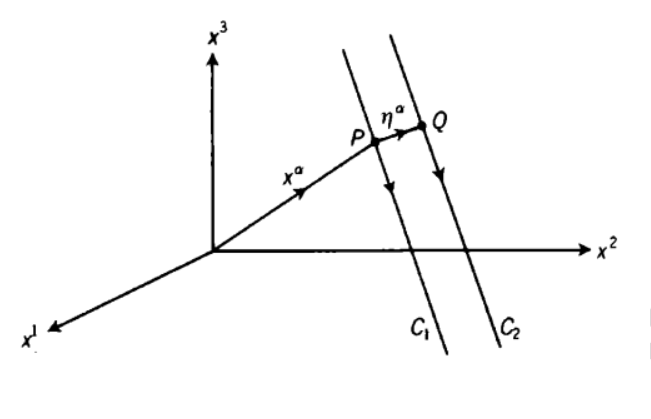
\includegraphics[scale=0.6]{deviation}
  \caption{Freely falling gravitational test particles at time t}
  \label{fig:deviation}
\end{figure}
Let 2 particles travel on curves $C_1$ and $C_2$ so that they reach the points P and Q at time t (Fig. 4.1). If we use the time t as the parameter along the 
curves, then the parametric equations of $C_1$ are $x^{\alpha}=x^{\alpha}(t)$
and those of $C_2$ are $x^{\alpha}=x^{\alpha}(t)+\eta^{\alpha}(t)$
If we define $\tensor{K}{^\alpha_\beta}$ by
$\tensor{K}{^\alpha_\beta}=\tensor{K}{_\beta^\alpha}=\partial^\alpha\partial_\beta \Phi $(where $\partial^\alpha=\delta^{\alpha\beta}\partial_\beta$). By using this notation we can deduce Newtonian geodesic equations to-
\begin{align}
    \dfrac{D^2\eta^\alpha}{D\tau^2}+\tensor{K}{^\alpha_\beta}&=0\\
    \tensor{K}{^\alpha_\beta}&=-\tensor{R}{^a_{bcd}}\tensor{e}{^\alpha_a}v^bv^c\tensor{e}{_\beta^d}
\end{align}
\subsection{The energy-momentum tensor}
\subsubsection*{Incoherent matter}
We start by considering the simplest kind of matter field, namely, that of non-
interacting incoherent matter or dust. Such a field may be characterized by 
two quantities, the 4-velocity vector field of flow $u^a(x) $ $\rho_0=\rho_0(x)$. Let us define the energy-momentum tensor $T_{ab}$ as
\begin{equation}
   T^{ab}=\rho_0u^au^b 
\end{equation}
We can prove that $\partial_b T_{ab}=0$ this equation is equivalent to conservation of 4-momentum(which means both energy and momentum are combined). If we use a non-flat metric in special 
relativity, then is replaced by its covariant counterpart
$$\nabla_b T_{ab}=0$$

\subsubsection{Perfect fluid}
A perfect fluid is characterized by three quantities: a 4-velocity $u^a=\dfrac{dx^a}{d\tau}$;a proper density field $\rho_0 = \rho_0$; and a scalar pressure field $p = p(x)$. In the
limit as $p$ vanishes, a perfect fluid reduces to incoherent matter. This suggests that we take the energy-momentum tensor for a perfect fluid to be of the form
\begin{equation}
    T^{ab}=(\rho_0+p)u^au^b-pg_{ab}
\end{equation}



\subsubsection{Maxwell energy-momentum tensor}
In order to write the Maxwells equations in tensorial form, we define an  
antisymmetric tensor $F^{ab}$, called \textbf{the electromagnetic field tensor} or Maxwell tensor, by
\begin{equation}
F^{ab}=  \begin{bmatrix}
0 & E_x & E_y & E_z\\
-E_x & 0 & B_z & -B_y\\
-E_y & -B_z & 0 & B_x\\
-E_z & B_y & -B_x & 0
\end{bmatrix}
\end{equation}
and the current density or source 4-vector $j^a$ by $j^a=(\rho,\textbf{j})$. Then maxwell's equations reduce to
\begin{align}
    \partial_b F^{ab}&=j^a\\
   \partial_{[a} F_{bc]} =\partial_a F_{bc}+\partial_c F_{ab}+\partial_b F_{ca}&=0
\end{align}
We define the \textbf{Maxwell energy-momentum tensor} as
\begin{equation}
    T^{ab}=\frac{1}{4\pi}(-g^{cd}F_{ac}F_{bd}+\frac{1}{4}g_{ab}F_{cd}F^{cd})
\end{equation}



\subsection{The weak-field limit}
We assume that there exists a privileged coordinate system $x^a=(ct,x,y,z)$ in which the metric $g_{ab}$ differs only slightly from the Minkowski metric $\eta_{ab}$. We also assume that the field is produced by bodies whose velocities are small compared with $c$. If v is a typical velocity of the 
bodies, then we let $\epsilon$ denote a small dimensionless parameter of order $\frac{v}{c}$ and our basic assumption is 
\begin{equation}
    g_{ab}= \eta_{ab}+\epsilon h_{ab}+O(\epsilon^2)
\end{equation}
For any function/ we assume the slow-motion approximation
\begin{equation}
    \epsilon\dfrac{\partial f}{\partial x^\alpha}\approx\dfrac{\partial f}{\partial x^0}
\end{equation}
Using these 2 approximations we can prove that in the \textbf{weak field limit}
\begin{equation}
g_{00}=1+\dfrac{2\phi}{c^2}+O(v/c)    
\end{equation}

\subsection{The Field Equations of GR}
The field equations of General Relativity are-
\begin{equation}
    G_{ab}=\dfrac{8\pi G}{c^4} T_{ab}=8\pi T_{ab}
\end{equation}
They can be viewed in three different ways
\begin{enumerate}
    \item The field equations are differential equations for determining the metric tensor $g_{ab}$ from a given energy-momentum tensor $T_{ab}$. This is a Machian way of viewing the equations since one specifies a matter distribution and then solves the equations to ascertain the resulting geometry. It is also a natural way of looking at the Einstein-Maxwell equations, namely, what geometry  corresponds to a given Maxwell tensor? The most important case of the equations is when $T_{ab}=0$, in which case we are concerned with finding vacuum solutions.
    \item The field equations are equations from which the energy-momentum tensor can be read off corresponding to a given metric tensor $g_{ab}$. It was originally thought that this would be a productive way of determining energy-momentum tensors. We simply choose arbitrarily ten functions of the coordinates, namely, the symmetric $g_{ab}$, and then we can compute $G_{ab}$ and read off $T_{ab}$. However, this rarely turns out to be very useful in practice because the resulting $T_{ab}$ are usually physically unrealistic. In particular, it frequently turns out that the energy density goes negative in some region, which we reject as unphysical because the positive character of energy density dominates gravitation theory.
    \item The field equations consist of ten equations connecting twenty  quantities, namely, the ten components of gab and the ten components of Tab. Hence, from this point of view, the field equations are to be viewed as constraints on the simultaneous choice of gab and Tab. This approach is used when one can partly specify the geometry and the energy-momentum tensor from physical considerations and then the equations are used to try and determine both quantities completely.
\end{enumerate}
The field equations are very difficult to handle because they are non-linear. 
Put another way, it means that you cannot analyse a complicated physical problem by breaking it up into simpler constituent parts. The non-linearity reveals itself physically in the following way: the gravitational field produced by some source contains energy and hence, by special relativity, mass, and this mass in turn is itself a source of a gravitational field. \textbf{The gravitational field is coupled to itself}. This non-linearity means that the equations are very difficult to solve in general. Indeed, originally Einstein anticipated that one would never be able to find 
an exact solution of them. 

\subsection{The cosmological term}
Einstein was rather sceptical about the full field equations and regarded the vacuum field equations as more fundamental. However, Einstein considered that even these equations were deficient in that they violated Mach's principle in the form M2, since they admit Minkowski space-time as a solution. This means that a test body in an otherwise empty universe would possess inertial properties (as all bodies do in special relativity) even though there is no matter to produce the inertia. In particular, he tried to find a static 
closed solution of the field equations corresponding to a universe uniformly 
filled with matter. In so doing, he found he was forced to modify the field 
equations by introducing an extra term, the cosmological term $\Lambda$, where $\Lambda$ is a constant called the cosmological constant, so that they become (with our sign conventions)
\begin{equation}
    G_{ab}-\Lambda g_{ab}=\dfrac{8\pi G}{c^4} T_{ab}=8\pi T_{ab}
\end{equation}
Since $\nabla_b g^{ab}=0$ it is consistent with the requirement $\nabla_b T^{ab}=0 $. Indeed, if, quite generally, we demand that the gravitational field equations should
\begin{enumerate}
    \item be generally covariant,
    \item be of second differential order in $g_{ab}$,
    \item involve the energy-momentum tensor $T_{ab}$ linearly,
\end{enumerate}
then it can be shown that the only equation which meets all of these 
requirements is 
$$R_{ab}+\mu Rg_{ab}-\Lambda g_{ab}=kT_{ab} $$
where $\mu$, $\Lambda$, and $k$ are constants. The demand that $T_{ab}$ satisfies the conservation equations $\nabla_b T_{ab}$ then leads to $\mu=-\frac{1}{2}$.

The constant $\Lambda$ is assumed to be very small in 
some sense and only of significance on a cosmological scale or on a quantum scale. 


\section{Schwarzschild metric and black holes}
\subsection*{Stationary solutions}
A metric will be stationary if there exists a special coordinate system in 
which the metric is visibly time-independent, i.e. 
\begin{equation}
    \dfrac{\partial g_{ab}}{\partial x^0}=^{*}0
\end{equation}
where $x^0$ is a timelike coordinate. We can show that if it satisfies in one coordinate then in all coordinates it satisfies-
\begin{equation}
    L_{X}g_{ab}=0
\end{equation}
\textit{A space-time is said to be stationary if and only if it admits a timelike Killing vector field.}
\subsection*{Hypersurface-orthogonal vector fields}
Let $f(x^a)=\mu$ be a family of hypersurfaces ,where different members of the family correspond to different values of $\mu$. If we define the covariant vector field $n_a=\dfrac{\partial f}{\partial x^a}$ to the family of hypersurfaces by 
\begin{equation}
    n_a=\dfrac{\partial f}{\partial x^a}
\end{equation}
Then $n_adx^a=g_{ab}n^adx^b=0$. It follows that $n_a$ is orthogonal to $S$(one of the hypersurfaces) and is therefore known as the normal vector field to $S$ at $P$. Any other vector field $X^a$ is said to be \textbf{hypersurface-orthogonal} if it is everywhere orthogonal to the family of hypersurfaces, in which case it must be proportional to $n_a$ everywhere, i.e.
\begin{equation}
    X^a=\lambda(x)n_a=\lambda f_{,a}
\end{equation}
We can show the following theorem
\begin{theorem}
Any non-null Killing vector field satisfying is necessarily hypersurface-orthogonal with $\lambda=X^2$
\end{theorem}
\subsection*{Static solutions}
If a solution is stationary, then, in an adapted coordinate system, the metric 
will be time-independent but the line element will still in general contain cross terms in $dx^0dx^\alpha$. If, in addition,the cross terms are absent, the metric is called \textbf{static}.The assumption that the solution is static means that $ds^2$ is invariant under a time reversal about any origin of time.
\begin{theorem}
A space-time is said to be static if and only if it admits a hypersurface- 
orthogonal timelike Killing vector field.
\end{theorem}
\begin{theorem}
In a static space-time, there exists a coordinate system adapted to the 
timelike Killing vector field in which the metric is time-independent and no cross terms appear in the fine element involving the time.
\end{theorem}
It can be shown that there still exists the coordinate freedom
\begin{align*}
    x^{'0}=Ax^0+B\\
    x^{'\alpha}=h'^\alpha(x^\beta)
\end{align*}
where $A$ and $B$ are constants and the functions $h^{'\alpha}$ are arbitrary. If the boundary conditions require $g_{00}\rightarrow1$ at spatial infinity, then this requires$A = +1$ . Neglecting time reversal, then this fixes A to be 1, and so we have defined a time coordinate, called \textbf{world time}, which is defined to within an unimportant additive constant. 




\subsection{Derivation of the Schwarzschild Solution}
The assumptions we take in this solution are-
\begin{enumerate}
    \item It is a spherically symmetric solution
    \item The electric charge of the mass, angular momentum of the mass, and universal cosmological constant are all zero. 
\end{enumerate}
Our starting ansatz, is that there exists a special coordinate system
$$(x^a)=(x_0,x_1,x_2,x_3)=(t,r,\theta,\phi)$$
in which the line element has the form 
$$ds^2=A(t,r)dt^2-2B(t,r)dtdr-C(t,r)dr^2-D(t,r)(d\theta^2+sin^2\theta d\phi^2) $$
where A, B, C, and D are as yet undetermined functions of $t$ and $r$.
If we introduce a new radial coordinate by the transformation $r\rightarrow r'=D^\frac{1}{2}$ then the line element becomes
$$ds^2=A'(t,r')dt^2-2B'(t,r')dtdr'-C'(t,r')dr^2-r^{'2}(d\theta^2+sin^2\theta d\phi^2) $$
Consider the differential 
$$A'(t,r')dt-B'(t,r')dr' $$
we can always multiply this by an integrating factor, $I=I(t,r')$ say, which makes it a perfect differential. We use this result to define a new time coordinate $t'$ by requiring-
\begin{align*}
    dt'&=I(t,r')[A'(t,r')dt-B'(t,r')dr']\\
\Rightarrow dt^{'2}&=I^2(A^{'2}dt^2-2A'B'dtdr'+B^{'2}dr^{'2})\\
\Rightarrow ds^2&=A'I^{-2}dt'^2-(C'-A^{'-1}B^{'2})dr^{'2}-r^{'2}(d\theta^2+sin^2\theta d\phi^2)
\end{align*}
Defining two new functions $\nu$ and $\lambda$ by(where $\nu=\nu(t,r)$) and $\lambda=\lambda(t,r)$
\begin{align*}
    A'I^{-2}&=e^{\nu}\\
    C'-A^{'-1}B^{'2}&=e^{\lambda}
\end{align*}
The definitions of v and A in (14.31) and (14.32) are given in terms of 
exponentials, which, since they are always positive, guarantees that the 
signature of the metric is $-2$. In fact, there are rigorous arguments which 
confirm that the most general spherically symmetric line element in four 
dimensions (with signature $-2$) can be written in the canonical form.
\begin{equation}
    ds^2=e^{\nu}dt^2-e^{\lambda}dr^{2}-r^{2}(d\theta^2+sin^2\theta d\phi^2)
\end{equation}
From the above line element we get-
$$ $$
\begin{align*}
    g_{ab}&=\text{diag}(e^{\nu},-e^{\lambda},-r^{2},-r^{2}sin^2\theta)\\
    g^{ab}&=\text{diag}(e^{-\nu},-e^{-\lambda},-r^{-2},-r^{-2}sin^{-2}\theta)
\end{align*}
If we denote derivatives with respect to t and r by dot and prime, respectively, then the non-vanishing components of the mixed Einstein tensor are
\begin{align}
     \tensor{G}{_0^0}&=e^{-\lambda}\left(\frac{\lambda'}{r}-\frac{1}{r^2} \right)+\frac{1}{r^2}\\
     \tensor{G}{_0^1}&=-e^{-\lambda}r^{-1}\dot{\lambda}=-e^{\lambda-\mu}\tensor{G}{_1^0}\\
     \tensor{G}{_1^1}&=-e^{-\lambda}\left(\frac{\nu'}{r}+\frac{1}{r^2} \right)+\frac{1}{r^2}\\
     \tensor{G}{_2^2}&=\tensor{G}{_3^3}=\frac{1}{2}e^{-\lambda}\left(\frac{\nu'\lambda'}{2}+\frac{\lambda'}{r}-\frac{\nu'}{r}-\frac{\nu^{'2}}{2}-\nu^{''}\right)+\frac{1}{2}e^{-\nu}\left(\ddot{\lambda}+\frac{\dot{\lambda}^2}{2}-\frac{\dot{\lambda}\dot{\nu}}{2}\right)
\end{align}
The contracted Bianchi identities reveal that equation (5.9) vanishes  
automatically if the first 3 equations all vanish. Hence, there are three independent equations to solve, namely,
\begin{align}
    e^{-\lambda}\left(\frac{\lambda'}{r}-\frac{1}{r^2} \right)+\frac{1}{r^2}&=0\\
    e^{-\lambda}\left(\frac{\nu'}{r}+\frac{1}{r^2} \right)-\frac{1}{r^2}&=0\\
    \dot{\lambda}=0
\end{align}
Adding 5.10 and 5.11-
\begin{align*}
    \lambda'+\nu'&=0\\
    \Rightarrow \lambda+\nu&=h(t)
\end{align*}
where h is an arbitrary function of integration. Here, A is purely a function of r by (5.12), and so (5.10) is simply an ordinary differential equation, which we write 
\begin{align}
    e^{-\lambda}-re^{-\lambda}\lambda'&=1\\
    \Rightarrow (re^{-\lambda})'=1\\
    \Rightarrow re^{-\lambda}=r+constant
\end{align}
Choosing the constant of integration to be $-2m$, for later convenience, we 
then obtain
$$e^{\lambda}=\left(1-\frac{2m}{r}\right)^{-1} $$
So, at this stage, the metric has been reduced, to
\begin{equation}
 g_{ab}=\text{diag}(e^{h(t)}\left(1-\frac{2m}{r}\right),-\left(1-\frac{2m}{r}\right)^{-1},-r^{2},-r^{2}sin^2\theta)
\end{equation}
The final stage is to eliminate $h(t)$. This is done by transforming to a new time coordinate $t'$ i.e. $t\rightarrow t'$ where $t'$ is determined by the relation
$$t'=\int^t_c e^{\frac{1}{2}h(u)}du$$
where c is an arbitrary constant. Then the only component of the metric which changes is $g^{'}_{00}=\left(1-\frac{2m}{r}\right)$. Dropping primes, we have shown that it is always possible to find a coordinate system in which \textbf{the most general spherically symmetric solution} of the vacuum field equations is
\begin{equation}
     ds^2=\left(1-\frac{2m}{r}\right)dt^2-\left(1-\frac{2m}{r}\right)^{-1}dr^2-r^{2}(d\theta^2+r^{2}sin^2\theta d\phi^2)
\end{equation}
This is the Schwarzschild line element. 
\subsection{Properties of the Schwarzschild solution }
We restrict attention to the exterior region $r>2m$ where the coordinates 
t and r are timelike and spacelike respectively. It is immediate from 
(5.17) that $g_{ab,0=^{*}0}$, and so the solution is stationary. We can also prove that it is static. This is stated as
\begin{theorem}[Birkhoff's theorem]
A spherically symmetric vacuum solution in the exterior region is necessarily static.
\end{theorem}
This is unexpected because in Newtonian theory spherical symmetry has 
nothing to do with time dependence. This highlights the special character of 
non-linear partial differential equations and the solutions they admit. If a spherically symmetric source is restricted to the region $r<a$ for some $a>2m$, then the solution for $r>a$ must be the Schwarzschild solution. However, the converse is not true: a source which gives rise to an exterior Schwarzschild solution is \textbf{not necessarily spherically symmetric}. If we take the limit of (5.17) as $r\rightarrow\infty$, then we obtain the flat space metric 
of special relativity in spherical polar coordinates. We have therefore shown that a spherically symmetric vacuum solution is \textbf{necessarily asymptotically flat}. 
Let us attempt an interpretation of the constant m appearing in the solution, by considering the Newtonian limit. A point mass M situated at the origin O in Newtonian theory gives rise to a potential $\phi=\dfrac{-GM}{r}$. Inserting this into the weak-field limit  gives
\begin{align*}
    g_{00}&\approx 1+\frac{2\phi}{c^2}=1-\frac{2GM}{c^2r}\\
    \Rightarrow m&=\frac{GM}{c^2}=M\text{(in relativistic units)}
\end{align*}

\subsection{Gravitational Singularities}
The Schwarzschild coordinates do not cover the axis $\theta= 0$, 
$\pi$ because the line element becomes degenerate there and the metric ceases to be of rank 4. This degeneracy could be removed by introducing Cartesian 
coordinates (x, y, z). Such points are called \textbf{coordinate singularities} because they reflect  deficiencies in the coordinate system used and are therefore removable. There are two other values of the coordinates for which the Schwarzschild solution is degenerate, namely, $r=2m$ and $r = 0$. The value r = 2m is known as the \textbf{Schwarzschild radius}($r_s$). The hypersurface r = 2m is a removable coordinate singularity. This is indicated by the Riemann tensor scalar invariant
$$R_{abcd}R^{abcd}=48m^2r^{-6}$$
which is finite at r = 2m. The singularity at the origin is irremovable and is variously called an \textbf{Gravitational, curvature, physical, essential,} or \textbf{real singularity}. The normal interpretation of the Schwarzschild solution is as a vacuum solution exterior to some spherical body of radius $a > 2m$. A different metric would describe the body itself for $r < a$, and would then correspond to some distribution of matter resulting in a non-zero energy-momentum tensor.

\subsection{Space-time diagrams}
We first consider the class of radial null geodesics defined by $ds^2=\dot{\theta}^2=\dot{\phi}=0$. Then using the geodesic equation given earlier we get(where a dot denotes differentiation with respect to an affine parameter u along the null geodesic)
$$\left(1-\dfrac{2m}{r}\right)\dot{t}^2-\left(1-\dfrac{2m}{r}\right)^{-1}\dot{r}^2=0$$
The Euler-Lagrange equation corresponding to a = 0 is
\begin{align*}
    \dfrac{d\left[\left(1-\dfrac{2m}{r}\right)\dot{t}\right]}{du}&=0\\
    \Rightarrow\left(1-\dfrac{2m}{r}\right)\dot{t}&=k\\
    \Rightarrow \dot{r}^2&=k^2\\
    \Rightarrow \dot{r}=\pm k
\end{align*}
from which it follows that r is an affine parameter.
\begin{align*}
    \dfrac{dt}{dr}&=\dfrac{\dot{t}}{\dot{r}}\\
    \Rightarrow\dfrac{dt}{dr}&=\dfrac{r}{r-2m}\\
    \Rightarrow t&=r+2mln|r-2m|+constant
\end{align*}
In the region I, by $r>2m$ r increases as t increases. We define the curves to be a congruence of \textbf{outgoing radial null geodesics}. Similarly, $r<2m$ gives the congruence of \textbf{ingoing radial null geodesics}. The diagram seems to suggest that an observer in region I moving in towards the origin would take an infinite amount of time to reach the Schwarzschild radius $r=2m$. It turns out that this space-time diagram is misleading, 
\begin{figure}[H]
    \centering
  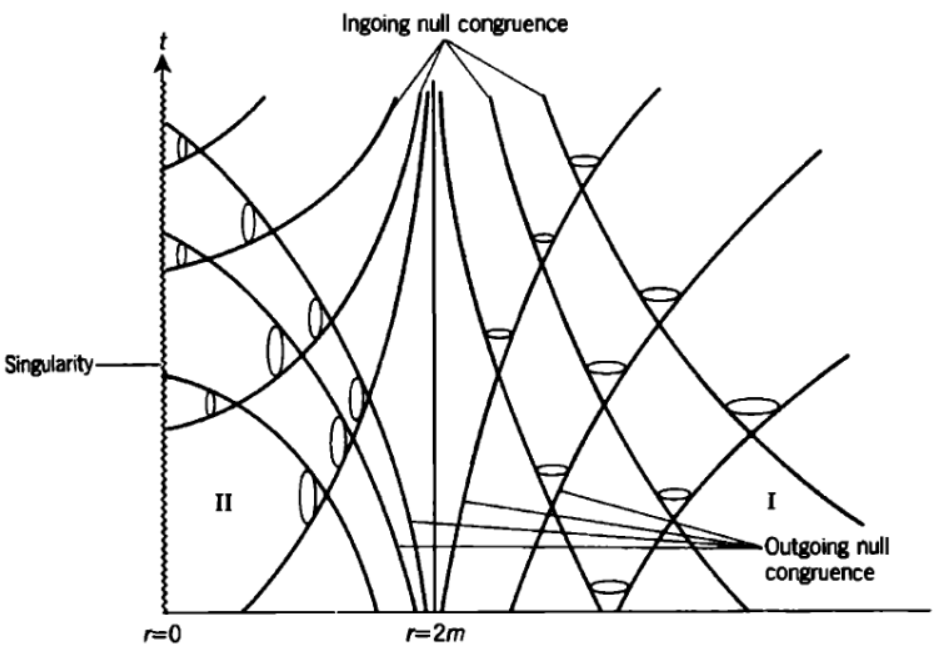
\includegraphics[scale=0.6]{st1}
  \caption{in Schwarzschild coordinates}
  \label{fig:deviation}
\end{figure}
Let us consider the path of a radially infalling free particle. It will move on a timelike geodesic given by the 2 equations(where a dot now denotes differentiation with respect to $\tau$)
\begin{align*}
\left(1-\dfrac{2m}{r}\right)\dot{t}^2-\left(1-\dfrac{2m}{r}\right)^{-1}\dot{r}^2&=1\\
\left(1-\dfrac{2m}{r}\right)\dot{t}&=1\\
\Rightarrow \left(\dfrac{d\tau}{dr} \right)^2&=\frac{r}{2m}\\
\Rightarrow \tau-\tau_0&=\frac{2}{3\sqrt{2m}}(r^{\frac{3}{2}}_0-r^{\frac{3}{2}})
\end{align*}
where the particle is at $r_0$ at proper time $t_0$. No singular behaviour 
occurs at the Schwarzschild radius and the body falls continuously to $ =0$ in a finite proper time. The coordinate $t$ is useful and physically meaningful asymptotically at large $r$ since it corresponds to the proper time measured by an observer at rest far away from the origin. From the point of view of such an observer, it takes an infinite amount of time for a test body to reach r = 2m. However, from the \textbf{point of view of the test body itself}, it reaches both $r=2m$ and $r=0$ in finite proper time. 
\begin{figure}[H]
    \centering
  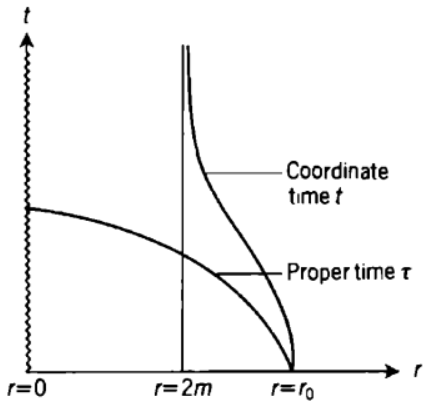
\includegraphics[scale=0.6]{st2}
  \caption{Radially infalling particle in  $\tau$ and $t$}
  \label{fig:deviation}
\end{figure}
\subsubsection*{Eddington-Finkelstein coordinates}
We are replacing $t$ with $\Bar{t}$ defined by $\Bar{t}=t+2mln|r-2m|$ then the line element becomes-
\begin{equation}
    ds^2=\left(1-\dfrac{2m}{r}\right)d\Bar{t}^2-\dfrac{4m}{r}d\Bar{t}dr-\left(1+\frac{2m}{r}\right)dr^2-r^{2}(d\theta^2+r^{2}sin^2\theta d\phi^2)
\end{equation}
\begin{figure}[H]
    \centering
  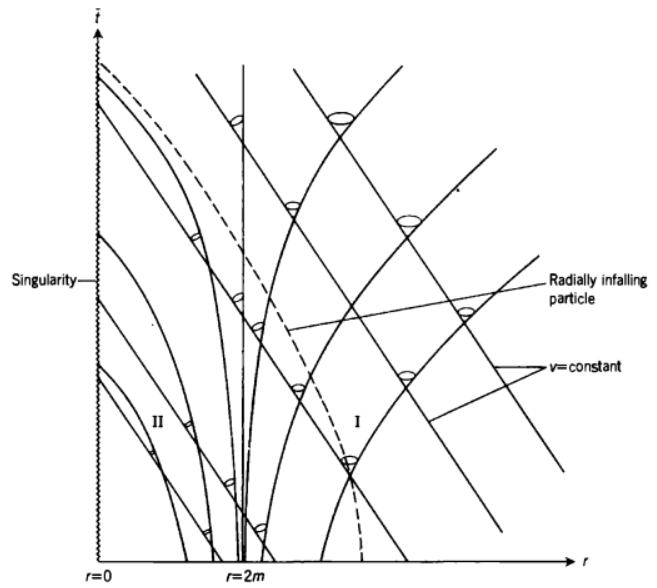
\includegraphics[scale=0.6]{st3}
  \caption{in Eddington-Finkelstein coordinates}
  \label{fig:deviation}
\end{figure}
\subsubsection*{Advanced Eddington-Finkelstein coordinates}
We are replacing $\Bar{t}$ with $\nu$ defined by $\nu=\Bar{t}+r$ then the line element becomes-
\begin{equation}
    ds^2=\left(1-\dfrac{2m}{r}\right)d\nu^2-2d\nu dr -r^{2}(d\theta^2+r^{2}sin^2\theta d\phi^2)
\end{equation}
\subsection{Neutral non-rotating black holes}
The Schwarzschild solution, taken to be valid for all $r>0$, is called a \textbf{Neutral non-rotating black hole} or \textbf{Schwarzschild black hole}.  We already have seen the space time diagrams for object whose entire solution is given by Schwarzschild metric. For much larger masses, General relativity predicts that a  spherically symmetric star will necessarily contract until all matter contained in the star arrives at a singularity at the centre of symmetry. 
\begin{figure}[H]
    \centering
  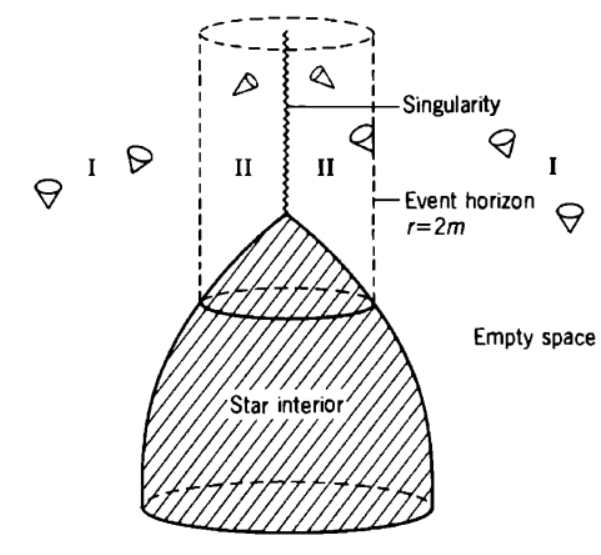
\includegraphics[scale=0.6]{st4}
  \caption{Gravitational collapse (one spatial dimension suppressed)}
  \label{fig:deviation}
\end{figure}
The surface $r=r_s=2m$ is called an \textbf{event horizon} because it represents the boundary of all events which can be observed in principle by an external inertial observer. Anything which passes through it will never come back because its \textbf{future cone} will completely point towards the singularity. We already saw that inside the event horizon the \textbf{timelike coordinate behaves as spacelike and the radial coordinate behaves as timelike}. Which means that inside event horizon future cones will always point towards singularity.
\subsubsection{Problems with Singularity}
We have only seen the solution of Neutral non-rotating black holes. But even in charged and rotating black holes event horizons and singularities exist. We might think other relativistic gravitational theories might not have singularities. However, Penrose and Hawking have managed to prove some remarkable theorems, called as singularity theorems, which suggest that many of the qualitative features of this collapse picture remain in a more general situation. Their results do not depend on the particular field equations of general relativity, but on much weaker assumptions such as the geometrical interpretation of gravity and the consequent curvature of space-time, relativistic causality, and the dominant energy conditions.(Refer 8.2 in Hawking and Ellis\cite{hae}).

Another important thing is the gravitational collapse deals with situations of high densities and that these are really the province of quantum theory. It seems likely that a classical theory like general relativity might be modified profoundly by quantum effects. Indeed, some theories of quantum gravity suggest that the collapse is halted before a singularity is reached. But as of now, there is still \textit{no complete and consistent quantum theory of gravity}.
\section*{Further reading}
\addcontentsline{toc}{section}{\protect\numberline{}Further reading}%
For the special relativity part I recommend the book Introduction to Special Relativity\cite{SR}. For GR if you want a good book for introduction read Introducing Einstein's Relativity\cite{dinv}. It is more intuitive and beginner friendly and is used as the main book for this. If you like mathematics more read General Relativity\cite{wald}. It is more advanced than the previous one.
If you like book full of anecdotes see Gravitation\cite{MTW}(it is considered as the bible for general relativists). It is a very lengthy book. And if you want a very advanced book read Hawking and Ellis\cite{hae} or S.Chandrasekhar\cite{SC}.

\printbibliography

\end{document}
